\documentclass{article}

\usepackage[english]{babel}
\usepackage[a4paper,top=2cm,bottom=2cm,left=3cm,right=3cm]{geometry}
\usepackage{amsmath}
\usepackage{graphicx}
\usepackage[colorlinks=true, allcolors=blue]{hyperref}
\usepackage{booktabs}
\usepackage{cleveref}
\usepackage{subcaption}
\usepackage{float}
\usepackage{parskip}
\title{Causal Inference for Dynamic Chemotherapy Treatment
Regimes}
\author{Jon Meksi, Jonas Limberg}

\begin{document}
\maketitle

\begin{abstract}
\noindent
This report studies chemotherapy regimen recommendation from observational longitudinal quality of life data, where counterfactual outcomes under alternative regimens are not observed. We preprocess lung cancer patient trajectories with EORTC QLQ-C30 measurements and compare five causal inference estimators: S-Learner, T-Learner, Backward Outcome Weighted Learning (BOWL), Causal Forest DML, and Dynamic DML, together with LSTM-based variants of the S- and T-Learner. The models are then evaluated on either equation-based semi-synthetic data or CRN-based semi-synthetic data. We also experiment with training and evaluating models on a large fully synthetic dataset. The CRN achieves better factual realism (RMSE 114 vs.\ 229, Pearson $r = 0.73$ vs.\ $r = 0.005$) but introduces a bias towards one treatment arm that inflates recommendation accuracy across all models in that benchmark, making it a rather unreliable discriminator. On the equation-based semi-synthetic benchmark, Causal Forest achieves the highest recommendation accuracy (40.2\%), but all models cluster near the random policy value baseline (117 days), confirming that the 438 row training set is insufficient for reliable causal estimation. On the fully synthetic benchmark (3000 test patients), DynamicDML leads with 70.4\% accuracy and a policy value of 248.05 (oracle 251.04, random 238.20), while the remaining estimators cluster between 55\% and 62\%. The results confirm that assigning a personalised regimen is doable at scale but remains challenging under the limited clinical dataset available.
\end{abstract}
\newpage

\tableofcontents
\newpage
\section{Introduction}
Choosing the right chemotherapy regimen for an individual cancer
patient is a difficult decision.  Depending on the patient's symptoms, treatment history, and current state, different regimens may result in varied outcomes. Observational data only records what happened under the regimen that was actually given.
The outcome under any alternative regimen (also known as \emph{counterfactual}) is unobserved and cannot be learned from the data
directly. This is the fundamental problem of causal inference, and
it makes standard supervised machine learning insufficient.
A model trained to predict observed outcomes will be biased by the fact that
treatment assignment in observational data is itself driven by the patients
state. Patients in worse condition often receive different regimens than
those in better condition, so a naive model will associate aggressive regimens with worse outcomes even when the regimen itself is not actually at fault.

Estimating these counterfactual outcomes is the central task of
\emph{causal machine learning}. This report documents the implementation and comparison of five
causal inference estimators for individualized chemotherapy treatment
effects, evaluated on a dataset of lung cancer patients with EORTC
QLQ-C30 quality of life measurements collected across multiple visits.
The models are: an S-Learner, a T-Learner, Backward Outcome
Weighted Learning (BOWL), Causal Forest DML, and Dynamic DML.
An LSTM-based regressor is additionally used as the base model for sequential variants
of the S and T-Learner, allowing them to use the patient's full
history rather than a cross-sectional snapshot. Because
counterfactual outcomes cannot be evaluated on real data, two
complementary semi-synthetic generators are used: A handcrafted
data generator that encodes its assumptions in explicit
equations, and a learned generator based on the Counterfactual
Recurrent Network (CRN) framework
\cite{bica2020estimatingcounterfactualtreatmentoutcomes}.
\section{Development}

\subsection{Use Case}
This work serves primarily as a research project to evaluate different
causal inference estimators on their ability to recover individualized
treatment effects from observational longitudinal clinical data.

The user is a researcher in causal machine learning. The input to the
system is a panel of patient visit records consisting of covariates
(EORTC QLQ-C30 subscales, gender, diagnosis, visit number), an assigned
regimen at each visit drawn from \{Cisplatin/Navelbine, Gemcitabine,
Docetaxel\}, and the observed outcome \texttt{time\_to\_last\_days}.
The output is, for each of the implemented estimators, a per-patient
ranking over the three regimens together with estimated treatment
effects $\hat{\tau}(x)$ for each pair of treatments.
\newline
The goal of the project is to characterize which
estimator family is most reliable on small, heterogeneous, longitudinal
clinical data, and to compare a handcrafted equation-based
counterfactual generator against a neural-network-based one.
\newline
Another goal of the project is to see the feasibility of using such
estimators for individualized chemotherapy regimen selection in lung
cancer. Choosing between regimens is rarely a decision with a single
correct answer. Patients differ in their symptom profiles and in the quality of life tradeoffs they
are willing to accept. The same regimen can lead to very different
trajectories in two patients with a similar disease. Current practice
relies on guidelines derived from average trial results and on the 
oncologist's personal experience, which is limited to the cases they
have seen. An estimator that produces reliable and specific
counterfactual outcomes for each patient from routinely collected data could let a
clinician compare the expected trajectories of the available regimens
for a specific patient and weigh them against the patient's own
preferences. Whether the estimators in this work are accurate enough on
small, noisy longitudinal data to support that kind of use is the
question that we aim to answer.

\subsection{Requirements}

\subsubsection{Functional Requirements}
Functionally, the pipeline imports raw patient visit records from CSV files and transforms them into a structured panel representation suitable for causal inference models. It preserves temporal order, keeps all visits from the same patient within a single split, normalizes chemotherapy regimen labels, restricts the analysis to the selected treatment arms, and encodes categorical variables numerically for downstream modeling. Missing covariate values are handled by the preprocessing and imputation procedure defined for the dataset, and the regression outcome \texttt{time\_to\_last\_days} is computed from the recorded visit dates and attached to each retained visit.

In addition to preprocessing the factual data, the pipeline supports counterfactual data generation. It produces semisynthetic outcomes using both the handcrafted generator and the CRN-based learned generator, and it also supports fully synthetic data generation for experiments in the absence of real patient records.

The modelling stage trains the implemented estimators, namely the S-Learner, T-Learner, BOWL, Causal Forest DML, Dynamic DML, and the LSTM variants of the S and T-Learner. For each evaluated patient visit, the system then produces either predicted potential outcomes for all treatment arms or a direct treatment recommendation, depending on the estimator type. Finally, it computes PEHE, ATE error, treatment recommendation accuracy, and policy value on semi-synthetic test data with known counterfactual outcomes, and generates comparison plots and table summaries of each model's performance.

\subsubsection{Non-Functional Requirements}
Reproducibility is the primary non functional requirement. The preprocessing, train/test split, model fitting, and evaluation pipeline are executable with fixed random seeds so that repeated runs have similiar results. Correctness and methodology consistency are more important than just the raw throughput, so the same preprocessing conventions, features, and evaluation protocol are applied across all the estimators.

Traceability is also important. Intermediate data products, predicted outcomes, recommendations, and evaluation summaries are all inspectable so that a reported result can be followed from the raw data to the final metric. The pipeline is also robust to small and unbalanced treatment groups, since the available clinical dataset contains few patients and uneven regimen frequencies, and so it supports longitudinal data without patient leakage or loss of the chronological structure.

From a software perspective, the implementation remains modular enough that additional estimators, generators, or evaluation metrics can be added without rewriting the full pipeline. It also runs on standard research hardware without needing specialised infrastructure, and training time is practical for multiple repeats on datasets of the size used in this project. Training time itself is therefore mostly bounded by dataset size.

\section{State of the Art}
We group the relevant prior work into methods that estimate treatment effects and
methods that generate the counterfactuals used to evaluate them.

\paragraph{Causal effect estimation}
Several families of estimators have emerged for recovering treatment effects from observational data. The simplest are metalearners, which split the task into ordinary prediction problems~\cite{K_nzel_2019}. The Causal Forest and the broader Double Machine Learning framework go a step further by first removing the part of the outcome and the treatment choice that the patient's features already explain, which keeps the estimated effect from being confused with baseline differences between patients and makes it robust to small modelling errors~\cite{chernozhukov2024doubledebiasedmachinelearningtreatment}, with a longitudinal version in Dynamic DML~\cite{lewis2021double}. Deep methods such as TARNet/CFR instead learn a patient representation in which treated and untreated groups look alike, reducing the bias a naive model would absorb from how treatments were assigned~\cite{shalit2017estimatingindividualtreatmenteffect}.

\paragraph{Counterfactual generation}
Handcrafted benchmarks such as IHDP fix the outcomes with a known equation, so the
true counterfactuals are available for scoring~\cite{shalit2017estimatingindividualtreatmenteffect}. Learned
generators like the Counterfactual Recurrent Network instead fit the outcome
dynamics from real trajectories, which produces more realistic counterfactuals on
longitudinal data~\cite{bica2020estimatingcounterfactualtreatmentoutcomes}.



\section{Material and Methods}

\subsection{Theoretical Background}
We work in the Rubin causel model framework. For a patient visit with covariates $X$ and an assigned treatment
$T \in \{0,\dots,K-1\}$ (here $K=3$), each arm $t$ has a potential outcome $Y(t)$,
the value \texttt{time\_to\_last\_days} would take if that arm were given. Only the
outcome under the assigned arm is observed,
\begin{equation}
    Y = Y(T),
\end{equation}
while the outcomes under the other arms remain counterfactual. This is the
fundamental problem of causal inference: only a single arm is
realised per visit, so individual treatment effects are never directly observed.

The quantity an estimator targets is the conditional average treatment effect (CATE)
of switching from arm $t_0$ to $t_1$,
\begin{equation}
    \tau(x) = {E}\!\left[\,Y(t_1) - Y(t_0) \mid X = x\,\right],
\end{equation}
which reduces to the average treatment effect (ATE) when averaging over the whole population. The
metrics in \Cref{sec:metrics} measure exactly these objects: PEHE scores the
estimated $\tau(x)$ at the individual level, ATE error its average. Because treatment
decisions here depend on the patient's trajectory, we use the longitudinal extension
in which the outcome at visit $v$ may depend on the whole treatment history
$\bar{T}_v = (T_0,\dots,T_v)$ rather than the current arm alone.

\subsection{Theoretical Assumptions}
\label{sec:assumptions}
Recovering CATE from observational data requires three standard
assumptions.

\textbf{Consistency} The observed outcome equals the potential outcome under
the assigned arm, $Y = Y(T)$, and no patient's outcome is affected by another
patient's treatment.

\textbf{Unconfoundedness.} Given the recorded covariates, treatment assignment is
independent of the potential outcomes.

\textbf{Positivity} Every patient has a non-zero probability of receiving
each arm.

In the longitudinal setting these become their sequential analogues: at each visit,
treatment is unconfounded and has positive probability given the observed history
$\bar{H}_{v-1}$ of past covariates, treatments, and outcomes. If these assumptions hold will be discussed in the discussion.


\subsection{Dataset}
The dataset consists of a CSV file of patient visit records collected during routine
clinical followup of lung cancer patients undergoing chemotherapy.  
Each row corresponds to one visit of a patient and the patients can be grouped by their ID.
The dataset centers on the chemotherapy regimens prescribed to the patient and the results from a EORTC Quality-of-Life Questionnaire (EORTC QLQ-C30). The answers are grouped by subscales and scored on a 0–100 scale. \cite{eortc_reference_values_2008}
The regression target \texttt{time\_to\_last\_days} used throughout this work is derived as the
number of days between a given visit and the patient's last recorded
visit. The treatment for a patient can end because they completed their treatment, they died or they quit due to personal reasons (health concerns, low quality of life, etc.).
Using our models we try to maximize the regression target which is contradictory for a cured patient, but the data does not show us the state of the tumor or any other symptoms. Thus, results should be interpreted with this ambiguity in mind.
\begin{table}[h]
\centering
    \begin{tabular}{lr}
        \toprule
        \textbf{Property}         & \textbf{Value} \\
        \midrule
        Total visits              & 996 \\
        Total patients            & 189 \\
        Deceased patients         & 90 \\
        Visits per patient (mean) & 5.3 \\
        Item columns              & 64 \\ 
        Subscale columns          & 16 \\
        \bottomrule
    \end{tabular}
    \caption{Summary of the chemotherapy QoL dataset. An item column corresponds to a questionnaire question.}
    \label{tab:dataset_summary}
\end{table}

\subsection{Basic Workflow}

\begin{figure}[!h]
    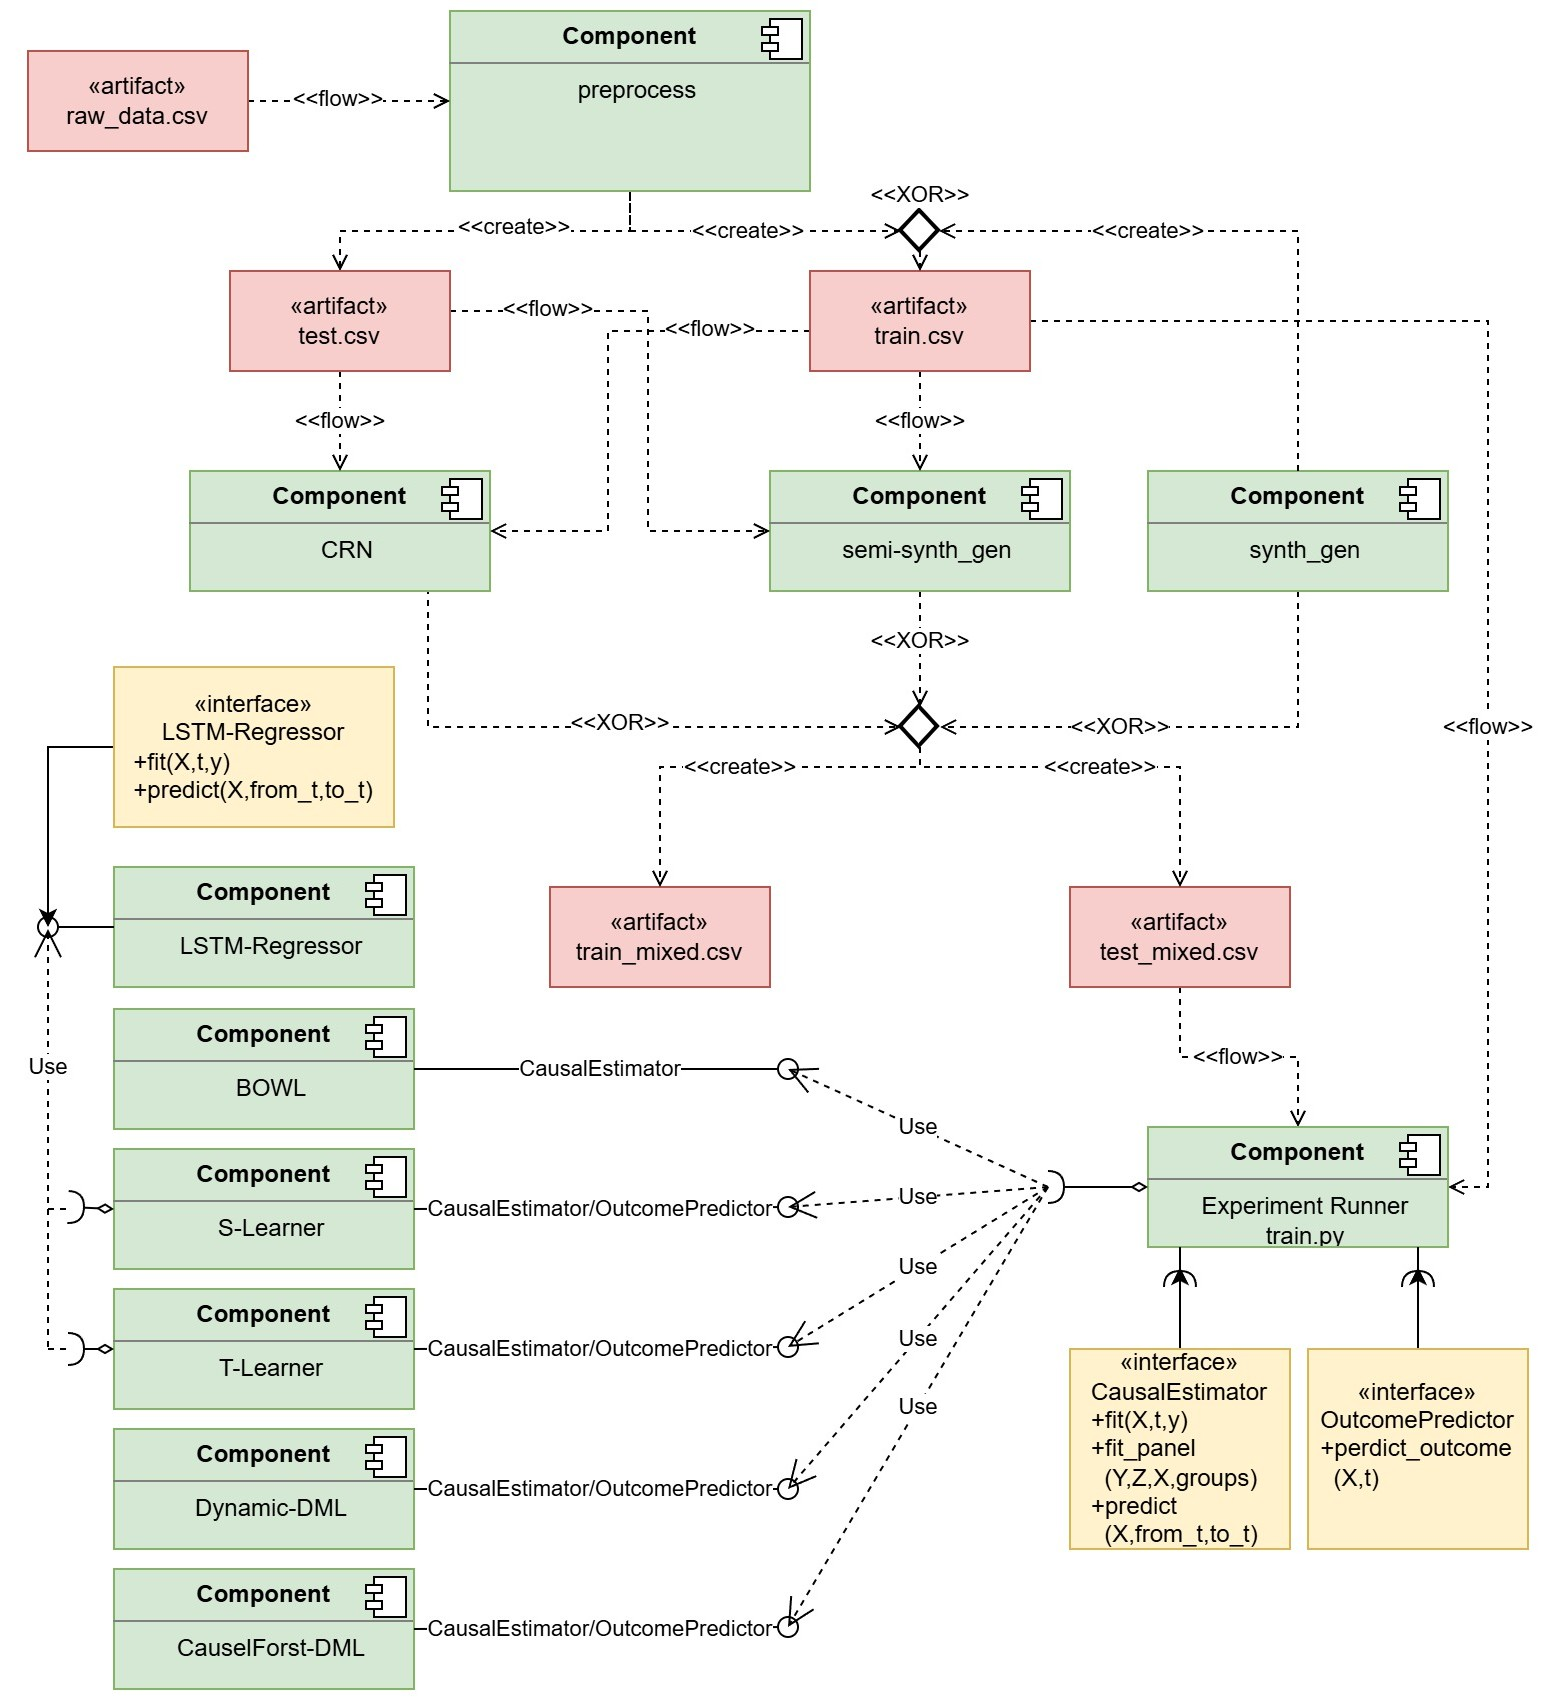
\includegraphics[scale=0.38]{images/component.jpg}
    \caption{Component diagram of the implementation. Preprocessing feeds either the CRN or the semi-synthetic generator, while the fully synthetic generator runs independently of the real data. The output of the selected generator is consumed by \texttt{train.py}. All five estimators provide the \texttt{CausalEstimator} interface and, except for BOWL, also \texttt{OutcomePredictor}. \mbox{S-Learner} and \mbox{T-Learner} additionally accept an \texttt{LSTMRegressor} through the \texttt{Regressor} interface.}
    \label{fig:component-diagram}
\end{figure}

The pipeline (\Cref{fig:component-diagram}) has four stages: preprocessing, counterfactual data generation, model fitting, and evaluation.

Preprocessing reads the raw CSV and produces a 
train and test split. Because counterfactual 
outcomes cannot be observed on real patients, the test split is 
passed through either the hand-crafted semi-synthetic generator 
or the CRN-based learned generator, which adds a counterfactual 
outcome for every treatment arm and writes the result to 
\texttt{test\_mixed.csv}. As an alternative, both the train 
and test split can be replaced entirely by the fully synthetic 
generator, which produces a fictional dataset without using 
any of the real records.

The experiment runner (\texttt{train.py}) loads \texttt{train.csv} 
and fits the five estimators. All five provide the 
\texttt{CausalEstimator} interface, which exposes \texttt{fit} for 
training on a feature matrix, treatment vector, and outcome vector, 
\texttt{fit\_panel} for the same with patient grouping for 
longitudinal data, and \texttt{predict} which returns the estimated 
individual treatment effect $\hat{\tau}(x)$ for switching from one 
treatment arm to another. Four estimators additionally provide 
\texttt{OutcomePredictor} with \texttt{predict\_outcome}, which 
returns the predicted outcome $\hat{\mu}_t(x)$ under a given 
treatment. BOWL is the exception because it returns a treatment 
recommendation rather than a per-arm outcome estimate, so an 
outcome predictor would not be meaningful for it.

To use the full visit history, the S-Learner and T-Learner accept 
a regressor through the \texttt{Regressor} interface. In the 
sequential variants this slot is filled by \texttt{LSTMRegressor}, 
which reads the patient's padded visit sequence one step at a 
time. BOWL, Causal Forest, and the non-sequential S- and T-Learner 
take a fixed-length history summary instead (mean, standard 
deviation, last value, previous value, and visit count per 
feature), computed inside \texttt{train.py} before fitting. 
Dynamic DML uses the panel structure throughout. It is trained on 
the full balanced panel and, at each evaluation step, queried with 
the patient's observed treatment history extended by the candidate 
treatment. Once the models are fitted, the runner evaluates them 
on \texttt{test\_mixed.csv} visit by visit, comparing the predicted 
best treatment against the counterfactual ground truth to compute 
the evaluation metrics.

\subsection{Data Pipelines}
\subsubsection{Preprocessing}
The goal of the preprocessing is to transform the raw dataset into a structured panel which is suitable for training causal-inference models. Three requirements
shape the preprocessing strategy. First, every treatment arm must be
represented in both the training and the test split, otherwise per-arm
estimators such as the T-Learner cannot be evaluated. Second, the
temporal structure of each patient's trajectory must be preserved, so
each patient is assigned entirely to one split and their visit sequence
is never divided between training and test.
Third, every retained row must carry information about both the temporal evolution of the patient and the treatment effect being estimated.
To achieve these requirements, parts of the 996 total visits in the raw dataset need to be removed.

27 patients only have one recorded visit in the dataset. These patients contribute a single row each with time\_to\_last\_days = 0 and no temporal signal, so they are removed.
Figure~\ref{fig:regimen_distribution} shows the distribution of the visits over the available regimens. Of the 29 distinct regimens only the three most frequent regimens (Cisplatin/Navelbine, Gemcitabine, Docetaxel) are used for the models. Figure~\ref{fig:regimen_distribution} suggests that the five most frequent regimens are a more natural cutoff point, but each additional arm enlarges the BOWL pairwise classifier
count ($\binom{K}{2}$) and the smallest pair would only contain 183 visits before splitting into the train and test set. With only three arms the smallest pair contains 284 visits.
This restriction comes with the trade-off: a patient's sequence may be truncated if they were prescribed any of the other 26 chemotherapy regimens at some point.


\begin{figure}[h]
    \centering
    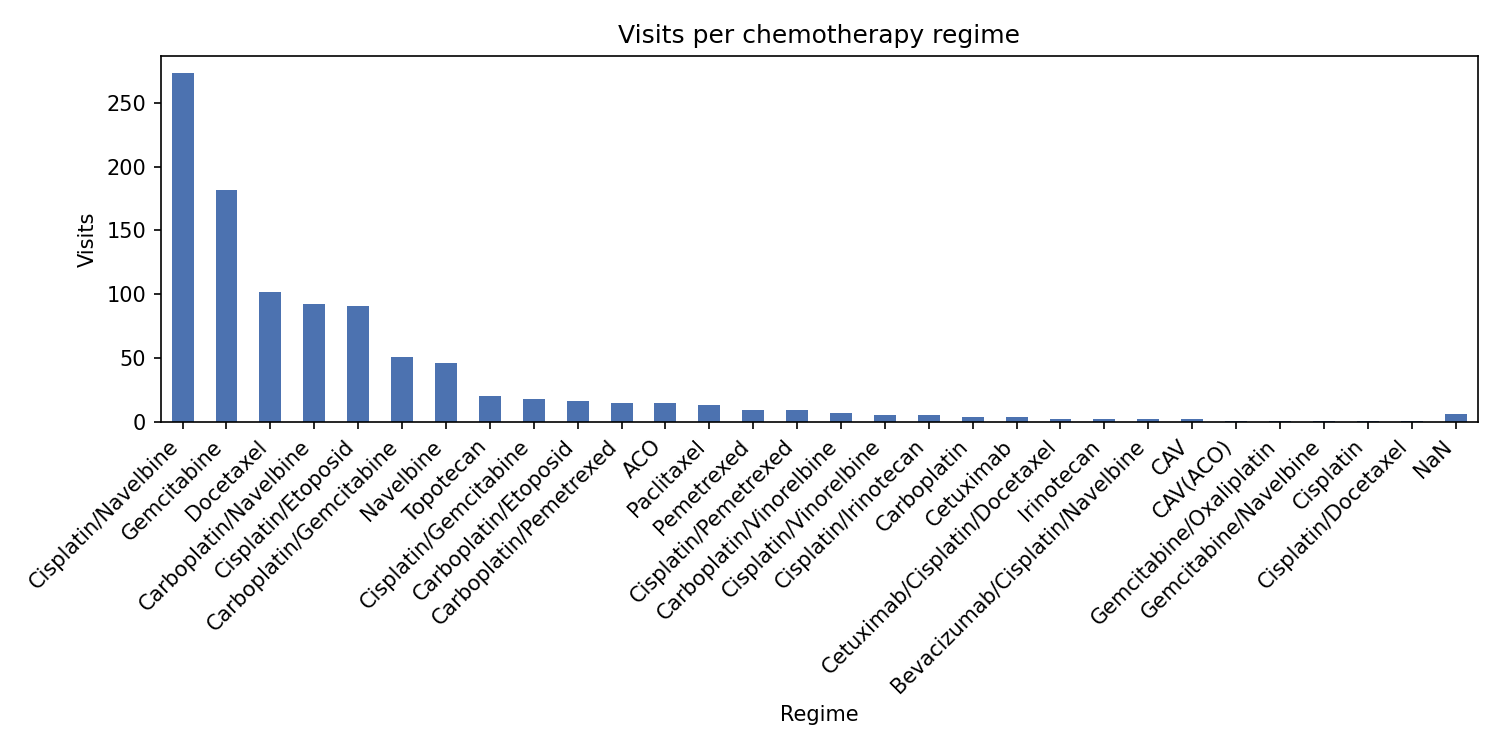
\includegraphics[width=0.95\textwidth]{images/regimen_distribution.png}
    \caption{Distribution of visits across chemotherapy regimens in the
        raw dataset. The single \texttt{NaN} entry corresponds to a visit
        with no recorded regimen.}
    \label{fig:regimen_distribution}
\end{figure}
Following preprocessing, which included regimen normalisation, the top-3
regimen filter, removal of single-visit patients, forward-fill
imputation of missing subscale values, label encoding of categorical
variables, and patient-level train/test splitting, the initial amount of 189 patients (996 visits) was reduced to 88 patients (535 visits). This final dataset was partitioned into a training set of 70 patients (438 visits) and a test set of 18 patients (97 visits). The retained feature set is restricted to ten EORTC QLQ-C30 subscales (physical, role, emotional, and cognitive functioning, global quality of life, fatigue, nausea/vomiting, pain, sleep disturbances, and appetite loss) together with encoded gender, initial diagnosis, and visit number, since the small data size cannot support a higher-dimensional feature space without risking overfitting. With only 18 test patients, per-arm test metrics carry substantial sampling variance, and absolute performance numbers should be interpreted accordingly.

\subsubsection{Semi-Synthetic Generation} \label{semisynth}
Evaluating causal-inference models on real data has fundamental
limitations. For each patient visit, only one outcome for the actually
assigned regimen is observed, and the counterfactual outcomes under
the other regimens remain unknown. A common solution is to generate
\emph{semi-synthetic} data that preserves the real outcome under the
assigned treatment while simulating the counterfactuals for the
remaining treatments.

The hand-crafted generator models a per-patient hidden state $h_v$
that evolves across visits and controls the average outcome at each
visit. At the first visit, $h_v$ is initialised from two components:
a baseline health score derived from the patient's EORTC QLQ-C30
subscales and an anchor derived from the patient's real
outcomes across their full trajectory. At every subsequent visit,
$h_v$ is updated from the next visit's baseline score, the previous
visit's real outcome, a treatment-specific carry term, and Gaussian
noise.

For each treatment, a treatment-specific offset is added to $h_v$
according to a fixed combination of the current visit's subscales,
so the same regimen helps a patient with one symptom profile and
hurts a patient with another. The synthetic outcome is drawn from a
gamma distribution whose mean is determined by the modified $h_v$.
The gamma distribution is chosen because it is positive and
right-skewed, which matches the heavy right tail of
\texttt{time\_to\_last\_days}.

The synthetic outcomes are then calibrated to the real outcome distribution by linear quantile matching at the 10th, 50th, and 90th percentiles, which aligns the distributions while preserving the rank ordering within each treatment arm.

The generator depends on the parameters that are hand-crafted and is therefore limited by the estimations of the designer. To complement this generator, a second semi-synthetic
generator is built on a learned encoder, described in
\Cref{sec:crn}.


\subsubsection{Counterfactual Recurrent Network}
\label{sec:crn}
The semi-synthetic generator in Section~\ref{semisynth} encodes its
data-generating process in equations chosen by hand. A better way to generate semi-synthetic data is a generator which learns from real factual outcomes,
a second counterfactual generator is built on the Counterfactual
Recurrent Network (CRN) framework of
Bica et al.~\cite{bica2020estimatingcounterfactualtreatmentoutcomes}.
The original CRN is a sequence-to-sequence model with an LSTM encoder
and an autoregressive decoder for multi-step rollouts. This work uses
only the encoder, since the downstream evaluation requires per-visit
counterfactuals rather than counterfactual sequences. \newline
At each visit $v$, the LSTM encoder reads the input

\begin{equation}
    \mathrm{input}_v \;=\; \bigl[\, x_v \,\Vert\, t_{v-1} \,\Vert\, y_{v-1}\,\bigr]
    \label{eq:crn_input}
\end{equation}
of the current features, the previous treatment, and the previous
outcome (zero-filled at $v=0$). The current treatment $t_v$ is
deliberately withheld from the encoder. The encoder produces a hidden
state $H_v$ that should encode the patient's state without encoding
which treatment they received. This addresses the problem that patients in worse condition tend to receive more aggressive treatments and also have worse outcomes regardless of treatment, so a naive model would learn a spurious negative association between aggressive treatments and outcomes. To prevent this, a
treatment classifier is attached to $H_v$ via a Gradient Reversal Layer. The classifier tries to recover $t_v$ from
$H_v$, while the Gradient Reversal Layer flips the sign of the gradient on the backward
pass, so the encoder is trained to make this prediction \emph{fail}.
The encoder is therefore optimizing two competing objectives simultaneously. It must produce a representation $H_v$
that is informative enough about the patient's prognosis for the outcome head to predict $y_v$ accurately, while being uninformative enough about the assigned treatment that the treatment classifier cannot recover $t_v$.
The equilibrium of this is a representation that retains as much prognostic information as possible while becoming identical across all regimens.
~\cite{bica2020estimatingcounterfactualtreatmentoutcomes}. 


\subsubsection{Fully Synthetic Data Generation}

When no real patient data is available, a fully synthetic set can be generated using \texttt{src/preprocess} \texttt{/synth\_gen.py}. The generator simulates individual patient trajectories without reference to any real records. This is just for experimenting and analyzing the efficiency of the models in the case of lack of sufficient real data.

Each synthetic patient is assigned a set of baseline EORTC QLQ-C30 subscale scores sampled from Gaussian distributions fitted to the real dataset's empirical means and standard deviations. Gender and diagnosis category are drawn uniformly, and a personal health trend (rate of deterioration per visit) is sampled from $\mathcal{N}(1.2,\ 0.4)$.

Each patient is simulated between 3 and 10 visits. The spacing between visits is drawn uniformly from $[14, 42]$ days. At every visit, covariate values drift from baseline according to the patient's trend and the subscale direction (functioning and quality-of-life scales decrease over time, symptom scales increase), with additive Gaussian noise.

Potential outcomes for all three treatment arms are computed at each visit from a linear combination of the current covariate values, remaining follow-up days, and arm-specific weights:
\begin{align}
    \mu_0(x) &\propto 35\,\text{phys} + 20\,\text{qol} - 25\,\text{fatigue} \\
    \mu_1(x) &\propto 45\,(1 - \text{pain}) + 15\,\text{emotional} - 10\,\text{phys} \\
    \mu_2(x) &\propto 50\,(1 - \text{fatigue}) + 15\,\text{role} - 20\,\text{sleep}
\end{align}
with independent Gaussian noise and clipping to $[0, 1500]$ days. The observed outcome is taken from the arm actually assigned. The remaining arms become the counterfactual ground truth.

Treatment assignment is covariate-informed: baseline physical functioning, fatigue, pain, role, and emotional functioning determine the logits of a softmax over the three arms, mixed with the empirical treatment frequencies from the real dataset (46\%, 18\%, 36\%). At each subsequent visit a switch probability is computed as $\text{clip}(0.03 + 0.0015\,r + 0.03\,v,\ 0.02,\ 0.35)$, where $r$ is the regret (difference between the best available potential outcome and the current arm's outcome) and $v$ is the zero-indexed visit number. When a switch occurs the new arm is sampled from a utility-weighted softmax with a penalty on returning to the current arm.

\subsection{Models}

Five causal inference models and a sequential LSTM used with two of them are implemented and compared. They share a common interface: \texttt{fit(X, T, y)}, \texttt{predict\_outcome(X, t)} and \texttt{predict(X, from\_t, to\_t)} where X is the per-visit feature matrix, T the assigned treatment, y the observed outcome (\texttt{time\_to\_last\_days}), and \texttt{predict} returns the estimated individual treatment effect (ITE) of switching from arm \texttt{from\_t} to arm \texttt{to\_t}, which shows the difference between the treatments. BOWL is the one exception: it produces a treatment recommendation only and does not implement \texttt{predict\_outcome}. The time steps of a sequence are indexed using v (\texttt{visit\_nr}).

\subsubsection*{S-Learner}

The S-Learner (single model learner) is one of the classical metalearners for heterogeneous treatment effect estimation. It fits a single regression model $\hat{\mu} : (X, T) \mapsto Y$, treating the treatment assignment $T$ as an additional input. In this formulation, the model learns a single response "area" over the joint space of patient covariates and treatment labels, so patients from all regimens contribute to one shared predictor. This sharing is good in small datasets because information from all arms is pooled instead of splitting the data into multiple arm-specific subsets.

If the base learner is written as $f_\theta(X, T)$, training amounts to minimizing the prediction loss over the factual data:

\begin{equation}
    \hat{\theta} \,=\, \arg\min_{\theta} \sum_{i=1}^{n} \ell\!\left(y_i, f_\theta(x_i, t_i)\right).
\end{equation}

Once the regression is fit, the CATE for switching from treatment $t_0$ to $t_1$ is estimated as the following:

\begin{equation}
    \hat{\tau}(x) = \hat{\mu}(x, t_1) - \hat{\mu}(x, t_0).
\end{equation}

Counterfactuals are therefore obtained by holding $X$ fixed and varying only the treatment indicator $T$. In implementation this is especially simple: the regressor is queried repeatedly with identical patient features and different treatment values appended. The main limitation is that if the base learner has a strong inductive bias toward smoothness, or if treatment is weakly represented relative to the covariates, the model may ignore treatment-specific interactions. In that case, the S-Learner tends to shrink the differences between regimens and can underestimate the actual heterogeneity in patient response.

\subsubsection*{T-Learner}

The T-Learner (two model learner) is another standard metalearner and can be seen as the opposite of the S-Learner. Instead of learning a single shared response surface, it fits a separate regression model $\hat{\mu}_t(X) \to Y$ for each treatment arm $t$, using only the observations that actually received treatment $t$. For $K$ regimens, this yields $K$ independently trained outcome models. Each model is free to learn its own nonlinear structure, which makes the method attractive when different therapies show genuinely different responses.

Training can be written as solving one regression problem per arm:

\begin{equation}
    \hat{\mu}_t \,=\, \arg\min_{g \in \mathcal{G}} \sum_{i: t_i=t} \ell\!\left(y_i, g(x_i)\right), \qquad t \in \{0,\dots,K-1\}.
\end{equation}

After these arm-specific models have been fit, the CATE is:

\begin{equation}
    \hat{\tau}(x) = \hat{\mu}_{t_1}(x) - \hat{\mu}_{t_0}(x)
\end{equation}

The T-Learner captures effect heterogeneity more explicitly than the S-Learner because interactions between patient state and treatment do not need to be represented through one shared model. Here that means each chemotherapy regimen can develop its own mapping from quality of life features and visit information to the predicted remaining follow up time. The tradeoff is data efficiency: when an arm has only a limited number of observations, its model must be estimated from that subset alone. There is no statistical sharing between arm models, so variance can increase substantially for underrepresented regimens and the resulting treatment effect estimates can be very unstable.

\subsubsection*{BOWL}

Backward Outcome Weighted Learning (BOWL) comes from the policy learning literature and approaches treatment selection as a classification problem rather than an outcome regression problem. Instead of estimating all potential outcomes and then comparing them, BOWL tries to learn a decision rule that directly maps patient covariates to the recommended treatment. The basic idea is that treatment assignments which led to better observed outcomes should receive more influence during training, while the propensity weighting corrects for the fact that some of the regimens are assigned more frequently than others.

For binary treatment, we can write the objective in terms of a decision function $f(x)$ and a policy $\pi(x)=\mathrm{sign}(f(x))$, with weights that are proportional to the inverse propensity-weighted outcome:

\begin{equation}
    w_i \propto \frac{y_i}{\hat{e}(t_i \mid x_i)}.
\end{equation}

For $K$ treatments, this implementation breaks the problem  down into $\binom{K}{2}$ pairwise binary classifiers. Each classifier between the arms $k$ and $l$ is trained only on visits belonging to those two arms, with larger weights assigned to patients whose observed regimen produced a larger outcome. By default, each pairwise problem is solved using an RBF-kernel SVM, which gives the method enough flexibility to represent nonlinear treatment boundaries.

At prediction time, the pairwise classifiers vote against one another and the final recommendation is obtained by plurality voting across all pairs. BOWL is therefore different from the other methods in this section: it does not estimate $\hat{\mu}_t(x)$ for every treatment. Its output is directly a policy recommendation. In this codebase the observed outcomes are also scaled to $[0,1]$ before weighting for numerical stability.

\subsubsection*{CausalForestDML}

The Causal Forest is a doubly robust CATE estimator based on the Double Machine Learning framework \cite{chernozhukov2018}. It further develops the idea of using random forests for nonparametric heterogeneity modeling. The goal is not just to predict patient outcomes, but to separate the effect of the treatment itself from differences in patient condition that also influence both treatment assignment and outcome.

Two nuisance models are first trained: one for the conditional outcome regression and one for the treatment assignment mechanism:

\begin{equation}
    m(x, t) \approx E[Y \mid X=x, T=t], \qquad e(x) \approx P(T \mid X=x).
\end{equation}

The method first explains as much of treatment assignment and outcome as possible using the observed patient features. It then compares the remaining unexplained parts, so the estimated treatment effect is less driven by baseline differences between patients and less sensitive to small errors in the first-stage models. A forest of trees then fits local treatment-effect models in regions of feature space containing similar patients, which allows the estimated effect $\tau(x)$ to vary across symptom profiles, diagnoses, and visit histories.

In the multi arm setting used here, effects are estimated relative to a specific reference treatment. A separate baseline outcome model is then fitted on that reference arm to recover the absolute potential outcomes:

\begin{equation}
    \hat{\mu}_t(x) = \hat{\mu}_{\mathrm{ref}}(x) + \hat{\tau}_{t,\mathrm{ref}}(x).
\end{equation}

This is useful because the forest focuses on estimating treatment contrasts, while the baseline regressor anchors those contrasts to an interpretable outcome scale. An advantage of Causal Forest over the simple metalearners is that it can also provide uncertainty intervals for the ITEs, which is valuable when treatment recommendations are made from sparse clinical data.

\subsubsection*{DynamicDML}

Dynamic DML extends the DML framework from cross sectional treatment effects to longitudinal or panel settings, where the current treatment decision depends on what happened earlier in the same patient's trajectory. This is important in chemotherapy data, because the regimen chosen at visit $v$ is influenced not only by the current symptoms, but also by prior treatments, prior outcomes, and the overall evolution of the disease. A method that ignores this temporal dependence risks attributing the effect of treatment history to the current regimen.

The model is fit on balanced longitudinal panels, where sequences of unequal length are brought to a uniform length through padding and truncation. If $Y_{i,v}$ denotes the outcome for patient $i$ at visit $v$, $T_{i,v}$ the treatment at that visit, and $H_{i,v-1}$ the observed history up to the previous visit, the dynamic setting can be written schematically as:

\begin{equation}
    Y_{i,v} = g(H_{i,v-1}, X_{i,v}, T_{i,v}) + \varepsilon_{i,v}.
\end{equation}

In the first stage, random forest nuisance models remove the confounding effect of past treatments and past outcomes on both the current treatment and the current outcome. The residuals from these partialled-out predictions are then used in the second stage, where a linear model estimates the CATE as a function of the patient's baseline features. This allows the model to make out the causal effect of the current treatment from the trajectory of prior treatments. When the input data is cross-sectional, each sample is treated as a single period panel so the model scales back down to standard DML. Constant variance features are automatically dropped before the final stage so that there is no rank deficiency.

Conceptually, Dynamic DML follows the same orthogonalisation logic as standard DML, but the nuisance models now condition on "lagged" information and panel structure. In this implementation the first stage is handled with Random Forest models for flexibility while the second stage uses a linear specification for the heterogeneous effect. That makes the final effect model easier to interpret and more stable on a small dataset.

\subsubsection*{Aggregate History}
The S/T-Learner, BOWL and  CausalForestDML are not sequential models and have no native ability to interpret the data in a time-series structure. A simple way to give them this ability is to summarize each patient's history into a fixed-length vector. In this implementation a handpicked subset of summary statistics is used. Libraries such as tsfresh compute around 800 of such features\cite{CHRIST201872}, but this amount would overwhelm the models since there would be more features than patients.
The aggregated history for a visit contains for each feature the mean and the standard deviation, for all visits until this point.
It also gets all the features for this visit and the previous visit.

\subsubsection*{LSTM using Metalearners}
The S- and T-Learner see only a single cross-sectional row at a time, and can incorporate previous visits only through the aggregated history features described above. An LSTM (Long Short-Term Memory) is a neural network which processes a sequence of features one step after another. For each step in the sequence it has one cell where it calculates an input gate $i_v$, a forget gate $f_v$, 
a candidate cell state $g_v$, an output gate $o_v$, the cell state 
$c_v$ and the hidden state $h_v$. (Eqs.~\eqref{eq:lstm_input}--\eqref{eq:lstm_hidden}).\cite{pytorch_lstm}

\begin{align}
    i_v &= \sigma\!\left(W_{ii}\,x_v + b_{ii} + W_{hi}\,h_{v-1} + b_{hi}\right)
        \label{eq:lstm_input}\\
    f_v &= \sigma\!\left(W_{if}\,x_v + b_{if} + W_{hf}\,h_{v-1} + b_{hf}\right)
        \label{eq:lstm_forget}\\
    g_v &= \tanh\!\left(W_{ig}\,x_v + b_{ig} + W_{hg}\,h_{v-1} + b_{hg}\right)
        \label{eq:lstm_candidate}\\
    o_v &= \sigma\!\left(W_{io}\,x_v + b_{io} + W_{ho}\,h_{v-1} + b_{ho}\right)
        \label{eq:lstm_output}\\
    c_v &= f_v \odot c_{v-1} + i_v \odot g_v
        \label{eq:lstm_cell}\\
    h_v &= o_v \odot \tanh(c_v)
        \label{eq:lstm_hidden}
\end{align}
$\sigma$ denotes the logistic sigmoid and $\odot$ the Hadamard product.
At each step the LSTM passes the previous cell state, the previous hidden state, and the current features into the next cell. The cell state corresponds to the "long-term memory" and holds information of the previous visits. The forget gate gives the LSTM the ability to erase irrelevant information from previous cells, so that the cell state doesn't grow too much for long sequences.\cite{818041}
$g_v$ represents the candidate cell and the input gate decides what information from $g_v$ gets passed to the cell state.~\eqref{eq:lstm_cell}
The hidden state corresponds to the "short-term memory" and the output gate decides what information of the cell state are relevant for it.~\eqref{eq:lstm_hidden}

\begin{figure}[h]
    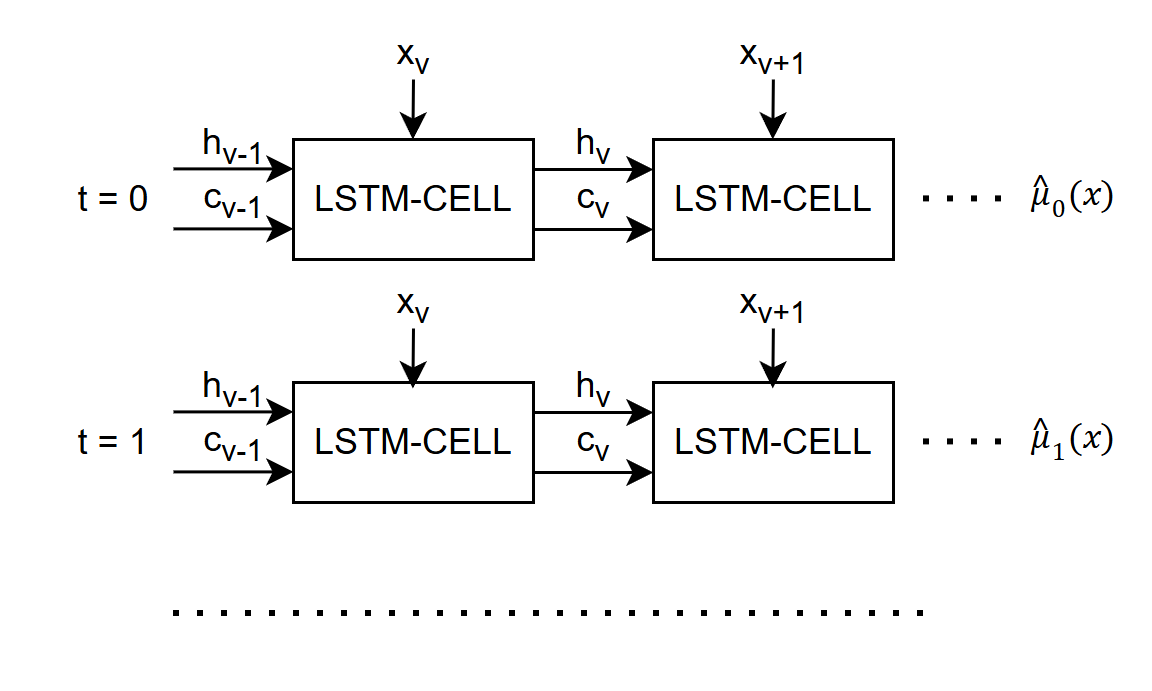
\includegraphics[scale=0.4]{images/LSTM-TLEARNER.png}
\caption{Unrolled LSTM computation for the T-Learner: each treatment arm
trains an independent LSTM that consumes the patient's visit sequence
and emits a treatment-specific outcome estimate $\hat\mu_t(x)$ at the
final step.}
\end{figure}

When the LSTM is used with a T-Learner, for each treatment a different LSTMs is trained and the last hidden state $h_{v_l}$ is used to calculate the predicted outcome. $W_l^{(t)}$ is the readout weight matrix and $b_l^{(t)}$ is the readout bias.

\begin{align}
    \hat{\mu}_t(x) &= W_l^{(t)}\, h_{v_l}^{(t)} + b_l^{(t)} \\
    \hat{\tau}(x)  &= \hat{\mu}_{t_1}(x) - \hat{\mu}_{t_0}(x)
\end{align}

When the LSTM is used with an S-Learner, a single LSTM is trained on all patients with the treatment $t$ appended to the input feature vector and counterfactual predictions are obtained by running the same network twice with different values of $t$. 
\begin{align}
    \hat{\mu}(x, t) &= W_l\, h_{v_l}(x, t) + b_l \\
    \hat{\tau}(x)   &= \hat{\mu}(x, t_1) - \hat{\mu}(x, t_0)
\end{align}




\section{Evaluation}
% TODO %

\subsection{Evaluation Protocol}
All models are evaluated on \texttt{test\_mixed.csv}, which 
contains the observed test patients together with the 
counterfactual potential outcomes $Y_0, Y_1, Y_2$ produced by 
one of the data generators. The evaluation is run visit by 
visit. For each patient and each visit $t$, the models receive 
the growing window of visits $0 \ldots t$ and produce 
predictions for that step.

How this window is consumed depends on the model. In the 
sequential setting, the LSTM variants of the S- and T-Learner 
receive the raw visit sequence padded to a fixed length and 
process it one step at a time through their recurrent cells. 
The non-sequential models (S-Learner, T-Learner, BOWL, and 
Causal Forest) cannot consume a sequence directly, so the 
growing window is collapsed into a fixed-length history 
summary containing the mean, standard deviation, last value, 
previous value, and visit count of each feature. Dynamic DML 
takes a third route. At each visit, the model receives the 
patient's first-visit feature row as the heterogeneity input 
and the observed past-treatment trajectory up to that step. 
The trajectory is padded to length \texttt{max\_periods} by 
continuing with the candidate treatment under evaluation.

For every visit, the true best treatment is defined as 
$\text{true\_best} = \arg\max_k Y_k^{\text{true}}$. The four 
outcome-predicting models additionally produce a predicted 
outcome $\hat{Y}_k$ for each treatment arm, from which a 
predicted best treatment $\hat{k}^* = \arg\max_k \hat{Y}_k$ is 
derived. BOWL skips the outcome step and returns a 
recommendation directly through its 
\texttt{predict\_optimal\_treatment} method. These per-visit 
predictions are the basis for the metrics described in 
\Cref{sec:metrics}.

\subsection{Metrics}
\label{sec:metrics}
The evaluation uses four complementary metrics. None of them are sufficient by themselves, because a model can estimate average effects well while failing to rank treatments for individual patients, or it can recommend the correct treatment frequently while badly estimating the magnitude of the underlying effect. Because of that the metrics are chosen to cover both effect estimation and treatment recommendation.

For models that predict potential outcomes for all treatment arms, the first metric is the Precision in Estimation of Heterogeneous Effects (PEHE). For a treatment pair $(t_0,t_1)$, the true individual treatment effect is

\begin{equation}
    \tau_i^{\text{true}} = Y_{i,t_1}^{\text{true}} - Y_{i,t_0}^{\text{true}},
\end{equation}

and the model prediction is

\begin{equation}
    \hat{\tau}_i = \hat{Y}_{i,t_1} - \hat{Y}_{i,t_0}.
\end{equation}

PEHE is then defined as

\begin{equation}
    \mathrm{PEHE} = \sqrt{\frac{1}{n} \sum_{i=1}^{n} \left(\hat{\tau}_i - \tau_i^{\text{true}}\right)^2 }.
\end{equation}

PEHE measures how accurately a model recovers patient-specific treatment differences. That makes it the main metric for heterogeneous effect estimation. A low PEHE means the model gets the treatment contrast right not only on average, but also at the individual-patient level.

The second metric is the absolute Average Treatment Effect (ATE) error. While PEHE focuses on individual-level heterogeneity, ATE error checks whether the model recovers the average effect over the whole evaluation set:

\begin{equation}
    \mathrm{ATE\ error} = \left| \frac{1}{n}\sum_{i=1}^{n} \hat{\tau}_i - \frac{1}{n}\sum_{i=1}^{n} \tau_i^{\text{true}} \right|.
\end{equation}

This metric is important because a model may have a somewhat bad PEHE but still estimate the overall effect correctly, or achieve a small average bias while missing substantial patient-level heterogeneity. Reporting both PEHE and ATE error distinguishes these two failure modes. Both metrics are computed separately for each unordered treatment pair. Since BOWL produces only treatment recommendations and not predicted potential outcomes, PEHE and ATE error are not defined for it.

The third metric is treatment recommendation accuracy. For each visit, the optimal treatment is the arm with the highest semi-synthetic ground-truth outcome,

\begin{equation}
    t_i^{\star} = \arg\max_t Y_{i,t}^{\text{true}},
\end{equation}

while the model recommendation is the arm with the highest predicted outcome,

\begin{equation}
    \hat{t}_i = \arg\max_t \hat{Y}_{i,t}.
\end{equation}

Accuracy is the fraction of evaluation steps for which the recommendation matches the true best arm:

\begin{equation}
    \mathrm{Accuracy} = \frac{1}{n} \sum_{i=1}^{n} \mathbf{1}\!\left[\hat{t}_i = t_i^{\star}\right].
\end{equation}

This is the most direct metric for the treatment-selection task, because it asks whether the model chooses the same regimen as the oracle. Unlike PEHE and ATE error, recommendation accuracy is also available for BOWL, since BOWL outputs a treatment policy directly.

The fourth metric is policy value. Instead of checking only whether the chosen arm matches the oracle, policy value measures the realised mean outcome under the model's decisions. For each visit, the outcome associated with the model's chosen treatment is taken from the semi-synthetic ground truth and then averaged over all visits:

\begin{equation}
    \mathrm{Policy\ Value} = \frac{1}{n} \sum_{i=1}^{n} Y_{i,\hat{t}_i}^{\text{true}}.
\end{equation}

Policy value is reported in the original outcome scale, here expected \texttt{time\_to\_last\_days}, and is therefore directly interpretable. A policy can have imperfect recommendation accuracy and still achieve a high policy value if its mistakes are clinically mild, while a policy with similar accuracy may have a much worse value if its errors are costly. For this reason policy value complements accuracy by measuring the quality of the decisions rather than only the rate of exact matches.

Taken together, PEHE and ATE error evaluate the quality of treatment-effect estimation, while recommendation accuracy and policy value evaluate the treatment policy. Lower values are better for PEHE and ATE error, and higher values are better for recommendation accuracy and policy value.

\section{Results}
\subsection{Generator Results}
The two semi-synthetic generators are evaluated by comparing the synthetic outcomes they produce under each visit's actually assigned treatment to the corresponding real outcomes. This factual comparison provides the only ground truth available, since the counterfactual outcomes under alternative treatments are unobservable in real clinical data.
The generators are evaluated on factual realism, which is measured with root mean squared error (RMSE), the mean absolute error (MAE) and the Pearson correlation coefficient. Lower RMSE and MAE values indicate more accurate predictions, since they show the deviation between a factual value and the predicted value. The Pearson correlation coefficient measures how strongly the factual and the generated outcomes follow the same trend. The closer the Pearson correlation coefficient is to one, the stronger the linear relationship between the generated and observed outcomes.
The CRN achieved a better factual prediction performance with a lower RMSE (114.05 vs.\ 229.11) and MAE
(69.93 vs.\ 146.24), as well as a much higher Pearson correlation
($r = 0.73$ vs.\ $r = 0.005$) compared to the equation-based generator.
Figure~\ref{fig:factual_scatter_generators} shows that the CRN predictions follow the observed outcomes more closely, whereas the equation-based generator shows little correlation with the factual values.

In addition to factual realism, distributional realism is measured by comparing the distribution of generated outcomes with the distribution of the observed outcomes. This is done using the Kolmogorov-Smirnov (KS) test, which measures the maximum distance between the empirical cumulative distribution functions of the two samples. A smaller KS statistic indicates that the two distributions are more similar. The corresponding p-value is used to test whether the difference between the distributions is statistically significant, where a high p-value suggests that the generated and real distributions are not significantly different.
The equation-based generator reproduced the overall outcome
distribution more accurately, with no significant difference detected
by the KS test ($p = 0.68$, KS statistic $= 0.1031$). In contrast, the CRN generator differed
significantly from the observed distribution ($p = 0.003$, KS statistic $= 0.2577$).

The results indicate a clear trade-off between the two generators. The equation-based generator achieves better distributional realism, as the generated outcomes closely match the overall empirical distribution. In contrast, the CRN demonstrates higher factual realism, providing more accurate predictions at the individual patient level.
However, the CRN shows a notable limitation in the counterfactual structure. It consistently assigns the highest predicted outcome to treatment 0 (Cisplatin/Navelbine). This indicates a strong bias in the learned policy, as the model tends to prefer a single treatment.


\begin{figure}[H]
    \centering

    \begin{subfigure}[b]{0.48\textwidth}
        \centering
        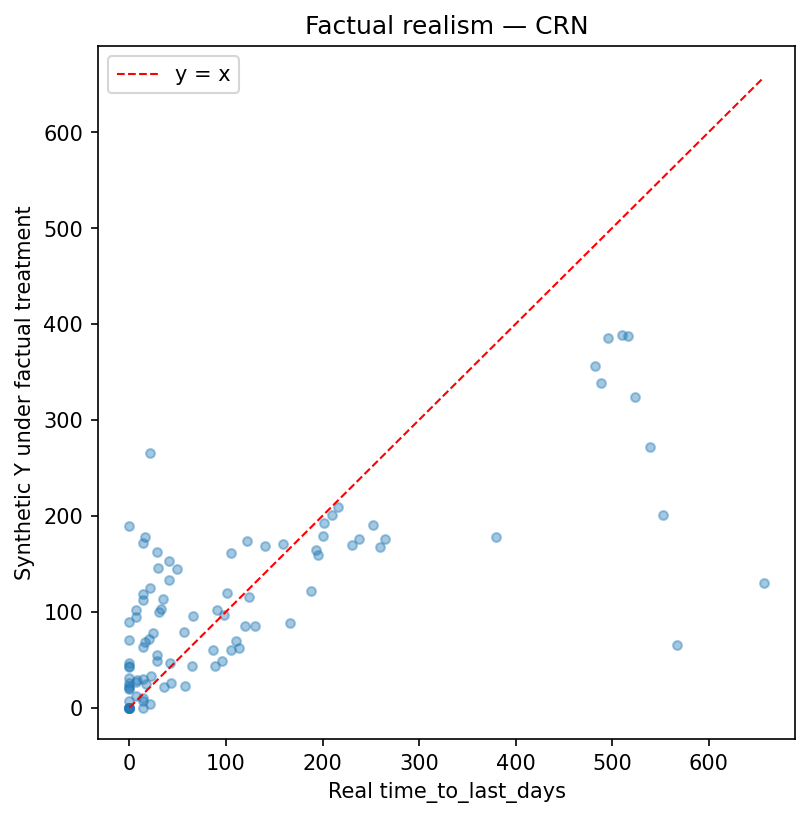
\includegraphics[width=\textwidth]{images/factual_scatter_CRN.png}
        \caption{CRN generator}
    \end{subfigure}
    \hfill
    \begin{subfigure}[b]{0.48\textwidth}
        \centering
        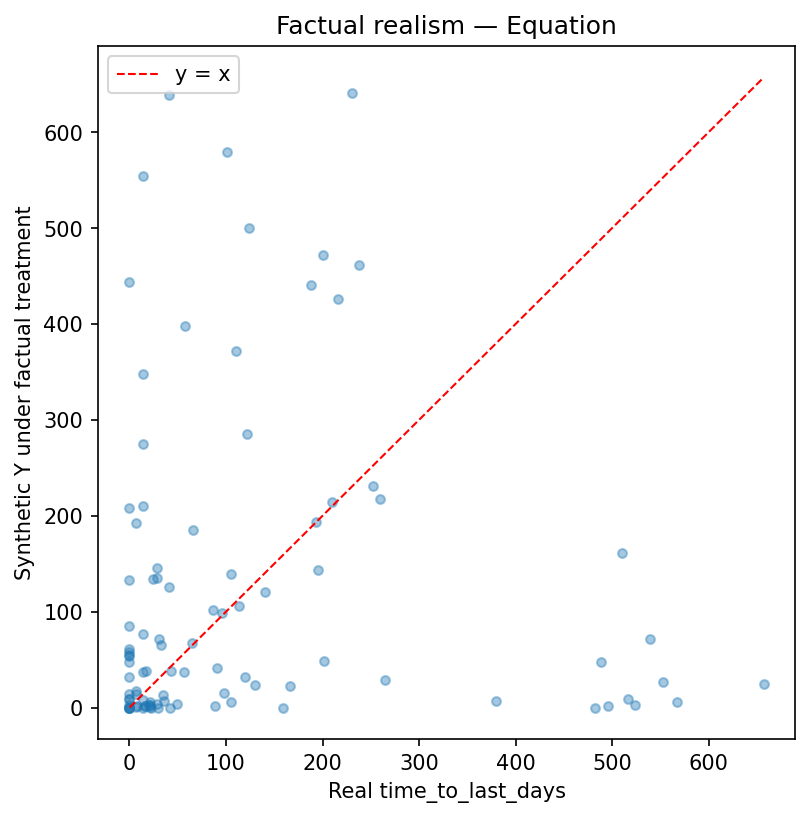
\includegraphics[width=\textwidth]{images/factual_scatter_Equation.png}
        \caption{Equation-based generator}
    \end{subfigure}

    \caption{Factual outcome prediction comparison between the CRN and equation-based generators. The x-axis shows the observed factual outcomes, while the y-axis shows the generated factual predictions.}
    \label{fig:factual_scatter_generators}
\end{figure}


\subsection{Model Results}


\subsubsection{Equation-based generator result}
\label{sec:res-eu}
For the equation-based semi-synthetic run, the training split contained
438 rows from 70 patients (6.3 visits/patient on average), and evaluation
was performed on 97 visit steps from 18 patients.

Due to small sample size PEHE values are high across all models , confirming that causal effect estimation from 438 rows is
underdetermined. Dynamic DML is most severely affected: the panel DML
estimator requires nuisance models converging at the $n^{1/4}$ rate
\cite{chernozhukov2016double,lewis2021double}, and with roughly 219 rows per
cross-validation this condition is far from met. As a result,
Dynamic DML produces the highest PEHE (266-320 across treatment pairs)
and the largest ATE errors (up to 90 for the $T_0$ vs.\ $T_1$ pair).
S-Learner and its LSTM version best approximate the true average treatment effects,
with ATE error values of 20.4 and 18.2 on the $T_0$ vs.\ $T_1$ pair.

Recommendation accuracy and policy value are summarised in
Table~\ref{tab:semi_model_summary}. Causal Forest achieved the highest
recommendation accuracy (40.2\%), followed by LSTM S-Learner and LSTM T-Learner (38.1\%
each), S-Learner (37.1\%), BOWL (34.0\%), T-Learner (30.9\%), and
Dynamic DML (29.9\%). Despite its poor effect estimates, Dynamic DML and
S-Learner achieved the highest policy values (122.70 and 122.49 days
respectively), most likely through coincidental alignment rather than accurate
causal estimation. The oracle value was 230.29 and the random baseline
was 117.08; the large gap between any model's policy value and the oracle
shows the difficulty of the task at this sample size.

\begin{table}[H]
    \centering
    \begin{tabular}{lcccc}
        \toprule
        \textbf{Model} & \textbf{Accuracy} & \textbf{Policy Value} & \textbf{PEHE $T_0$\,v\,$T_1$} & \textbf{ATE err $T_0$\,v\,$T_1$} \\
        \midrule
        Causal Forest & 40.2\% & 113.92 & 210.11 & 59.73 \\
        LSTM-S        & 38.1\% & 109.56 & 207.10 & 18.22 \\
        LSTM-T        & 38.1\% & 113.51 & 207.26 & 21.85 \\
        S-Learner     & 37.1\% & 122.49 & 206.68 & 20.40 \\
        BOWL          & 34.0\% & 105.96 & --     & --    \\
        T-Learner     & 30.9\% & 114.77 & 206.60 & 48.37 \\
        Dynamic DML   & 29.9\% & 122.70 & 266.52 & 90.35 \\
        \midrule
        Oracle        & --      & 230.29 & --     & --    \\
        Random        & --      & 117.08 & --     & --    \\
        \bottomrule
    \end{tabular}
    \caption{Model summary on the equation-based semi-synthetic evaluation set (97 steps, 18 patients). PEHE and ATE error are shown for the $T_0$ vs.\ $T_1$ treatment pair.}
    \label{tab:semi_model_summary}
\end{table}

Figure~\ref{fig:semi_model_plots} shows three diagnostics.
The PEHE comparison plot highlights the uniformly high error values
caused by sample size constraints and shows that Dynamic DML is a clear
outlier with substantially higher PEHE than the rest. The policy comparison plot
shows that all of the model policy values cluster near the random
baseline, far below the oracle. The ATE error plot shows that
S-Learner and its LSTM version recover the true average treatment effects the best on
this small training set.

\begin{figure}[H]
    \centering
    \begin{subfigure}[b]{1\textwidth}
        \centering
        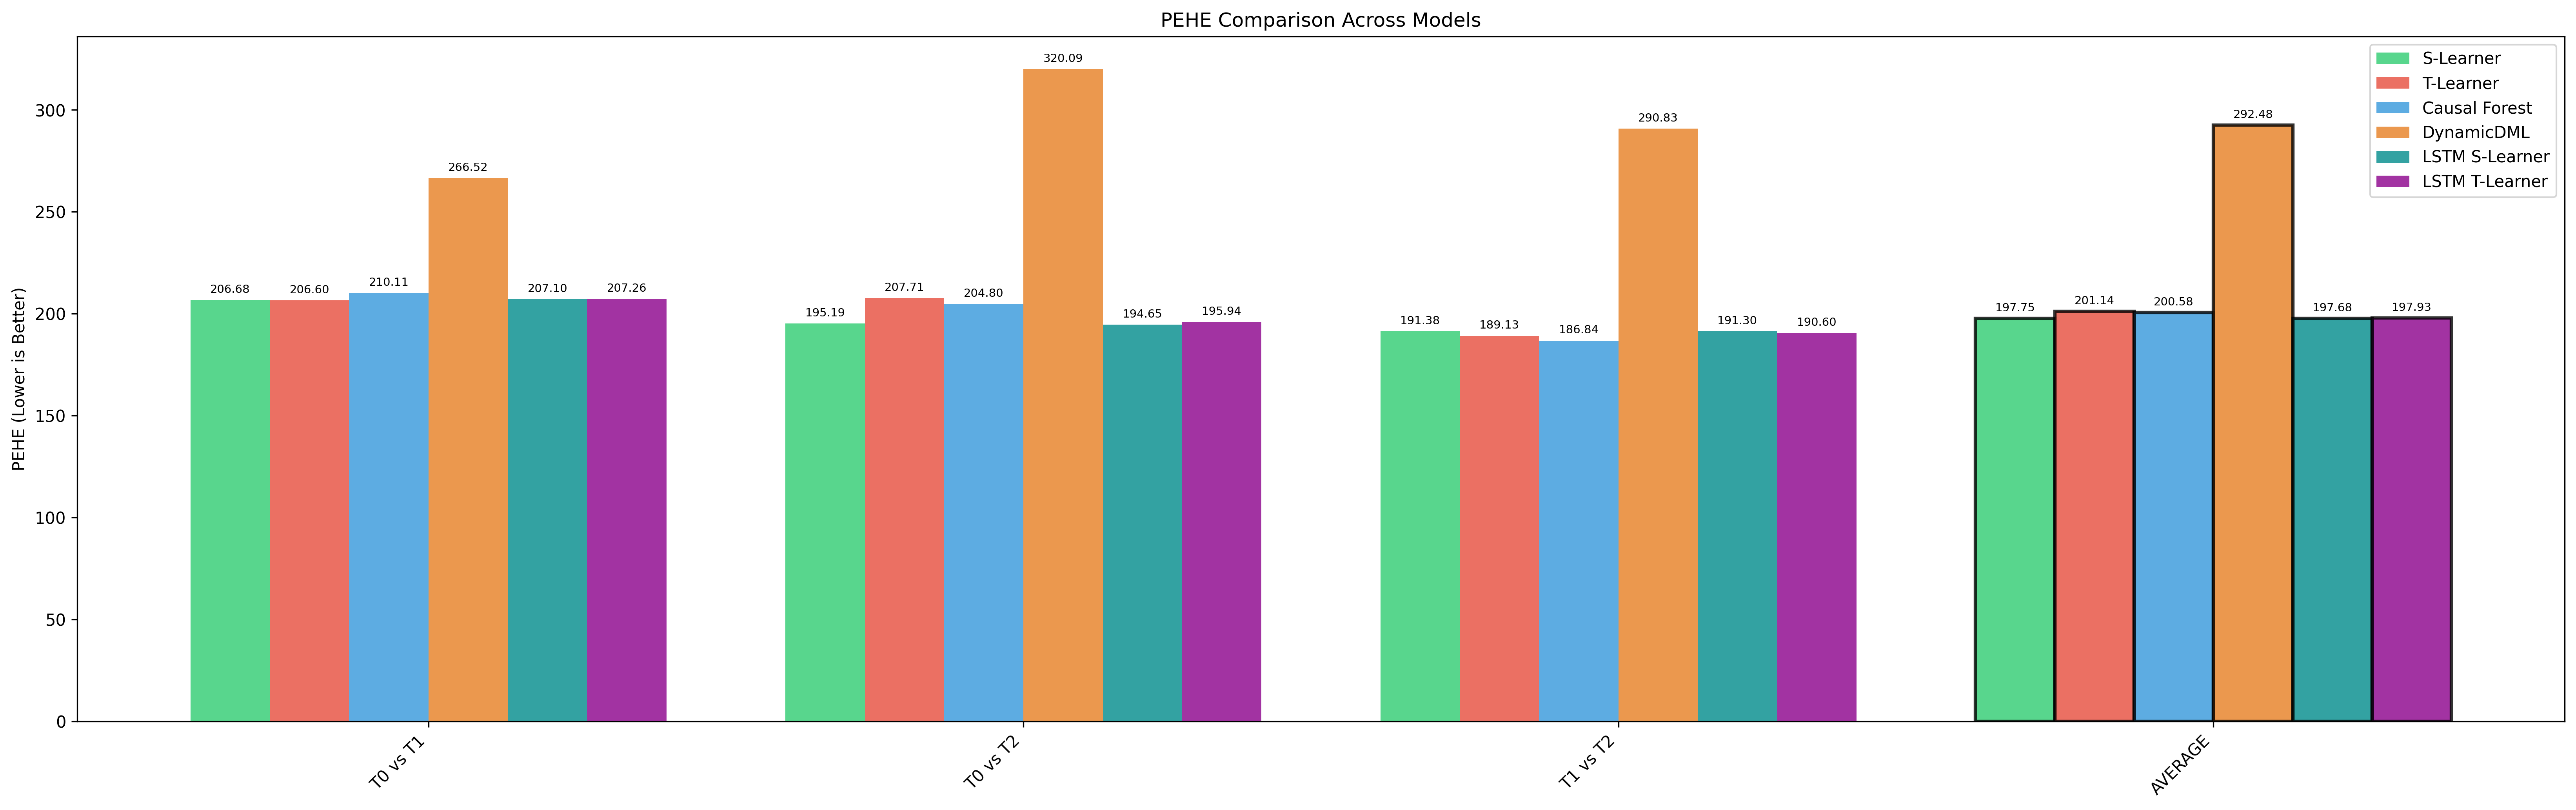
\includegraphics[width=\textwidth]{images/semisynth_pehe.png}
        \caption{PEHE by treatment pair}
    \end{subfigure}
    \\
    \begin{subfigure}[b]{1\textwidth}
        \centering
        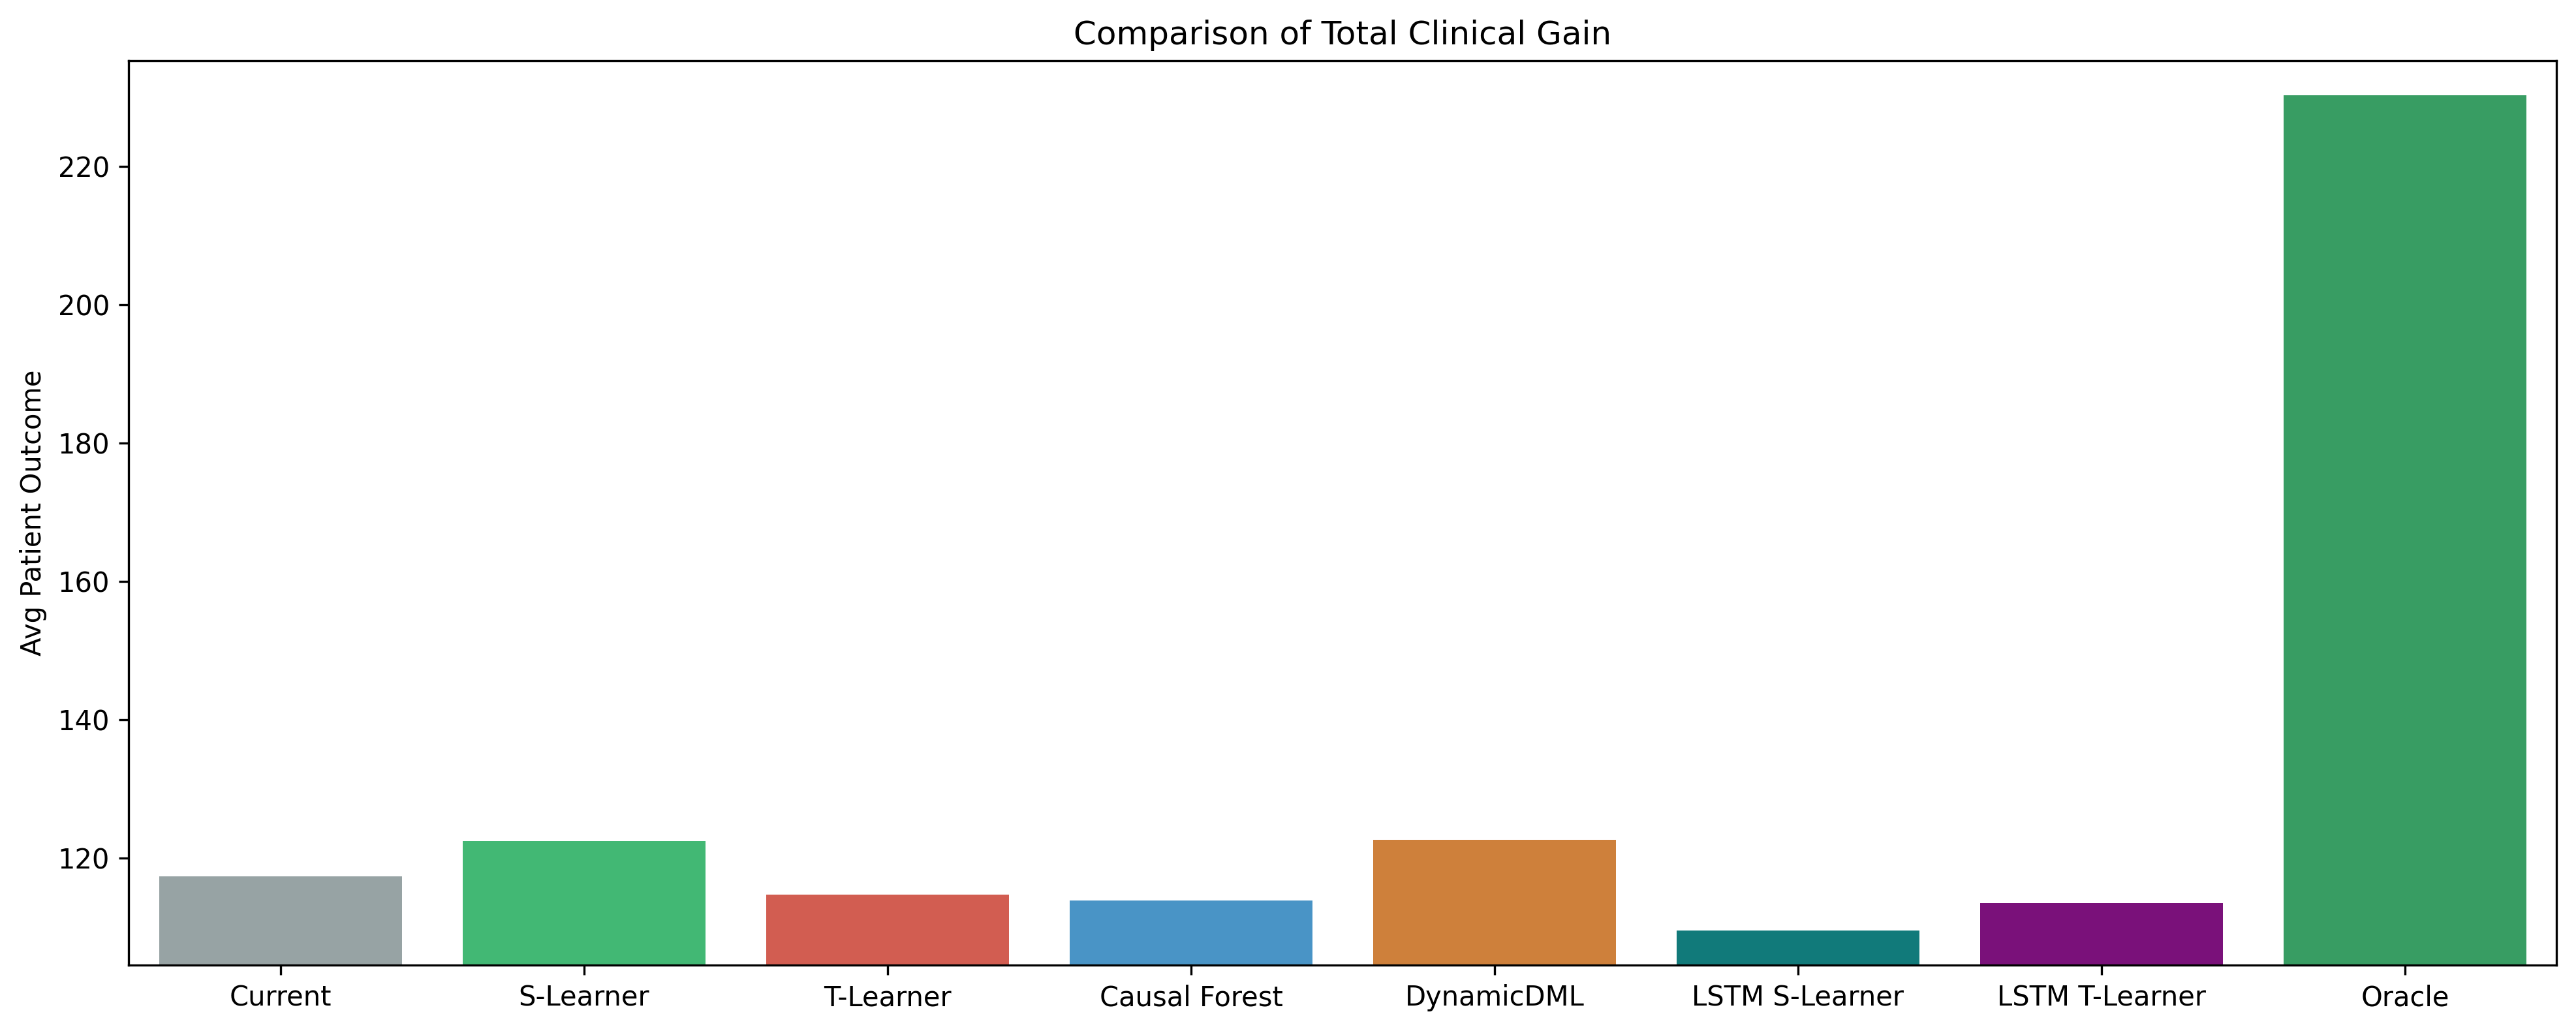
\includegraphics[width=\textwidth]{images/semisynth_policy.png}
        \caption{Policy value comparison}
    \end{subfigure}
    \\
    \begin{subfigure}[b]{1\textwidth}
        \centering
        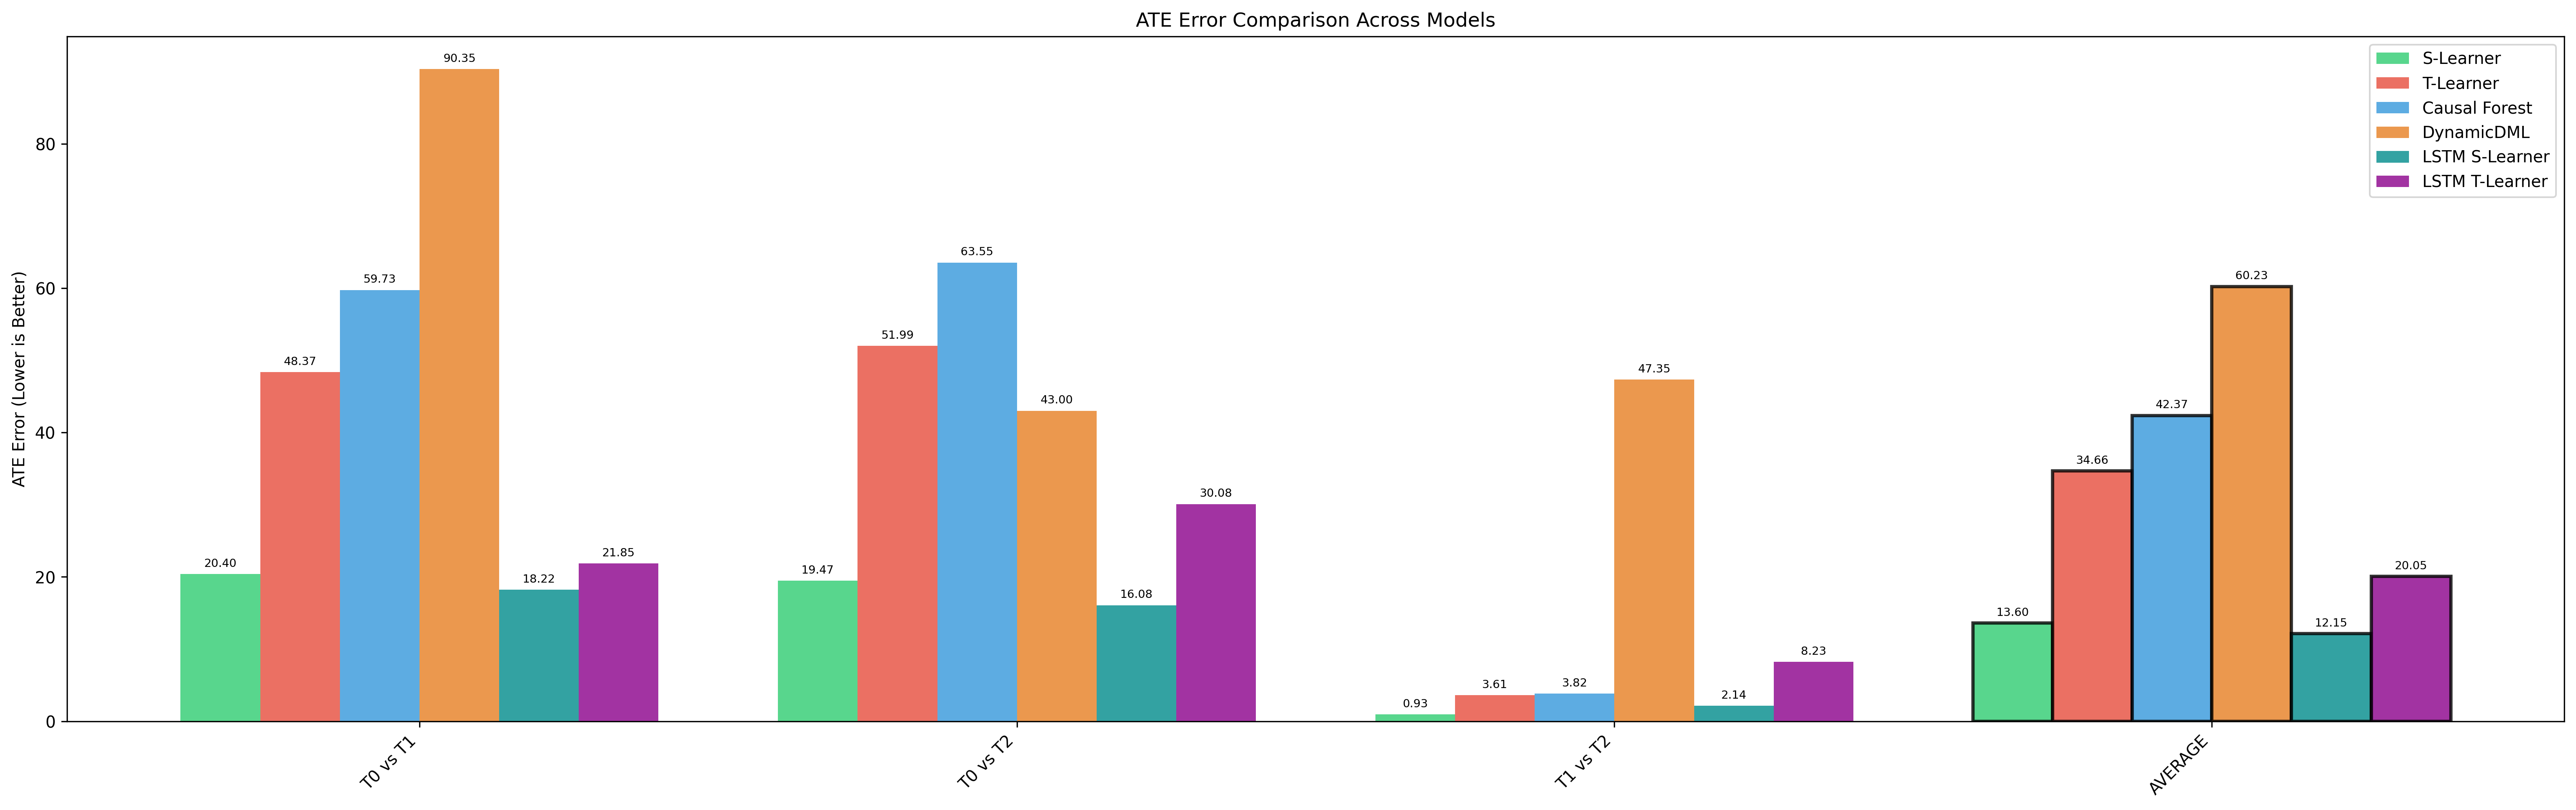
\includegraphics[width=\textwidth]{images/semisynth_ate.png}
        \caption{ATE error by treatment pair}
    \end{subfigure}
    \caption{Semi-synthetic equation-based model diagnostics (18 test patients).}
    \label{fig:semi_model_plots}
\end{figure}

\newpage
\subsubsection{CRN generator result}

The CRN-based semi-synthetic run covers the same input data and evaluation set. The CRN learns the counterfactual outcome distribution directly from real patient trajectories and produces more realistic counterfactuals than the equation-based generator, but it also has a
tendency to assign the highest predicted outcome to treatment
$T_0$ (Cisplatin/Navelbine). This bias inflates recommendation
accuracy for any model that mostly recommends $T_0$, making accuracy
less reliable as the sole discriminator in this setting.

Recommendation accuracy and policy value are summarised in
Table~\ref{tab:crn_model_summary}. The LSTM S-Learner achieved the highest recommendation
accuracy (97.9\%), closely followed by Causal Forest (95.9\%) and LSTM T-Learner
(93.8\%). The bias around $T_0$ is clearly shown for those models. S-Learner and BOWL (68.0\%)
and T-Learner (61.9\%) show intermediate accuracy, while Dynamic DML had the
lowest accuracy (51.5\%) and policy value (120.43). The oracle policy
value was 134.07 and the random baseline was 117.08.

For effect estimation, the LSTM T-Learner achieved the best PEHE on the $T_0$ vs.\ $T_1$
pair (11.90), with S-Learner (13.55) and LSTM-S (15.26) close behind.
Causal Forest was best on the $T_0$ vs.\ $T_2$ pair (20.45). Dynamic DML
again produced the highest PEHE (173--245 across pairs). ATE errors follow a
similar pattern: LSTM-T (11.25) and S-Learner (12.70) best recover the true
average $T_0$--$T_1$ treatment effect.

For uncertainty, we report the mean 95\% Confidence Interval (CI) width per treatment pair and model.
On both the equation-based and CRN-based runs, this metric does not change at all since we are measuring the same models and features. In both cases, Dynamic DML and T-Learner are much, wider than the other estimators, while the LSTM variants are the tightest.

\begin{table}[H]
    \centering
    \begin{tabular}{lccc}
        \toprule
        \textbf{Model} & \textbf{CI width $T_0$\,v\,$T_1$} & \textbf{CI width $T_0$\,v\,$T_2$} & \textbf{CI width $T_1$\,v\,$T_2$} \\
        \midrule
        S-Learner     & 15.3120 & 18.8903 & 6.3221 \\
        T-Learner     & 189.3371 & 173.7151 & 147.3197 \\
        Causal Forest & 117.8222 & 113.5618 & 123.1943 \\
        Dynamic DML   & 2585.8128 & 1231.9254 & 3142.3771 \\
        LSTM-S        & 3.4110 & 3.6241 & 3.6271 \\
        LSTM-T        & 4.0766 & 5.2947 & 4.9442 \\
        \bottomrule
    \end{tabular}
    \caption{Mean 95\% CI width on the semi-synthetic evaluation set (97 steps, 18 patients).}
    \label{tab:semi_ci_width}
\end{table}

\begin{table}[H]
    \centering
    \begin{tabular}{lcccc}
        \toprule
        \textbf{Model} & \textbf{Accuracy} & \textbf{Policy Value} & \textbf{PEHE $T_0$\,v\,$T_1$} & \textbf{ATE err $T_0$\,v\,$T_1$} \\
        \midrule
        LSTM-S        & 97.9\% & 133.25 & 15.26  & 14.89 \\
        Causal Forest & 95.9\% & 133.44 & 38.36  & 26.63 \\
        LSTM-T        & 93.8\% & 133.14 & 11.90  & 11.25 \\
        S-Learner     & 68.0\% & 128.88 & 13.55  & 12.70 \\
        BOWL          & 68.0\% & 125.58 & --     & --    \\
        T-Learner     & 61.9\% & 126.59 & 66.82  & 15.27 \\
        Dynamic DML   & 51.5\% & 120.43 & 173.26 & 57.25 \\
        \midrule
        Oracle        & --      & 134.07 & --     & --    \\
        Random        & --      & 117.08 & --     & --    \\
        \bottomrule
    \end{tabular}
    \caption{Model summary on the CRN-based semi-synthetic evaluation set (97 steps, 18 patients). PEHE and ATE error are shown for the $T_0$ vs.\ $T_1$ treatment pair.}
    \label{tab:crn_model_summary}
\end{table}

Figure~\ref{fig:crn_model_plots} shows the PEHE comparison, policy value
diagnostics, and ATE error comparison. The PEHE plot shows that
LSTM-T and S-Learner achieve substantially lower errors than the other
models on the $T_0$ vs.\ $T_1$ pair, while Dynamic DML is an order of
magnitude higher. The policy value plot shows LSTM-based models
clustering near the oracle. The ATE error plot confirms that
LSTM-T and S-Learner best recover the true average treatment effects from
the CRN-generated outcomes.

\begin{figure}[H]
    \centering
    \begin{subfigure}[b]{1\textwidth}
        \centering
        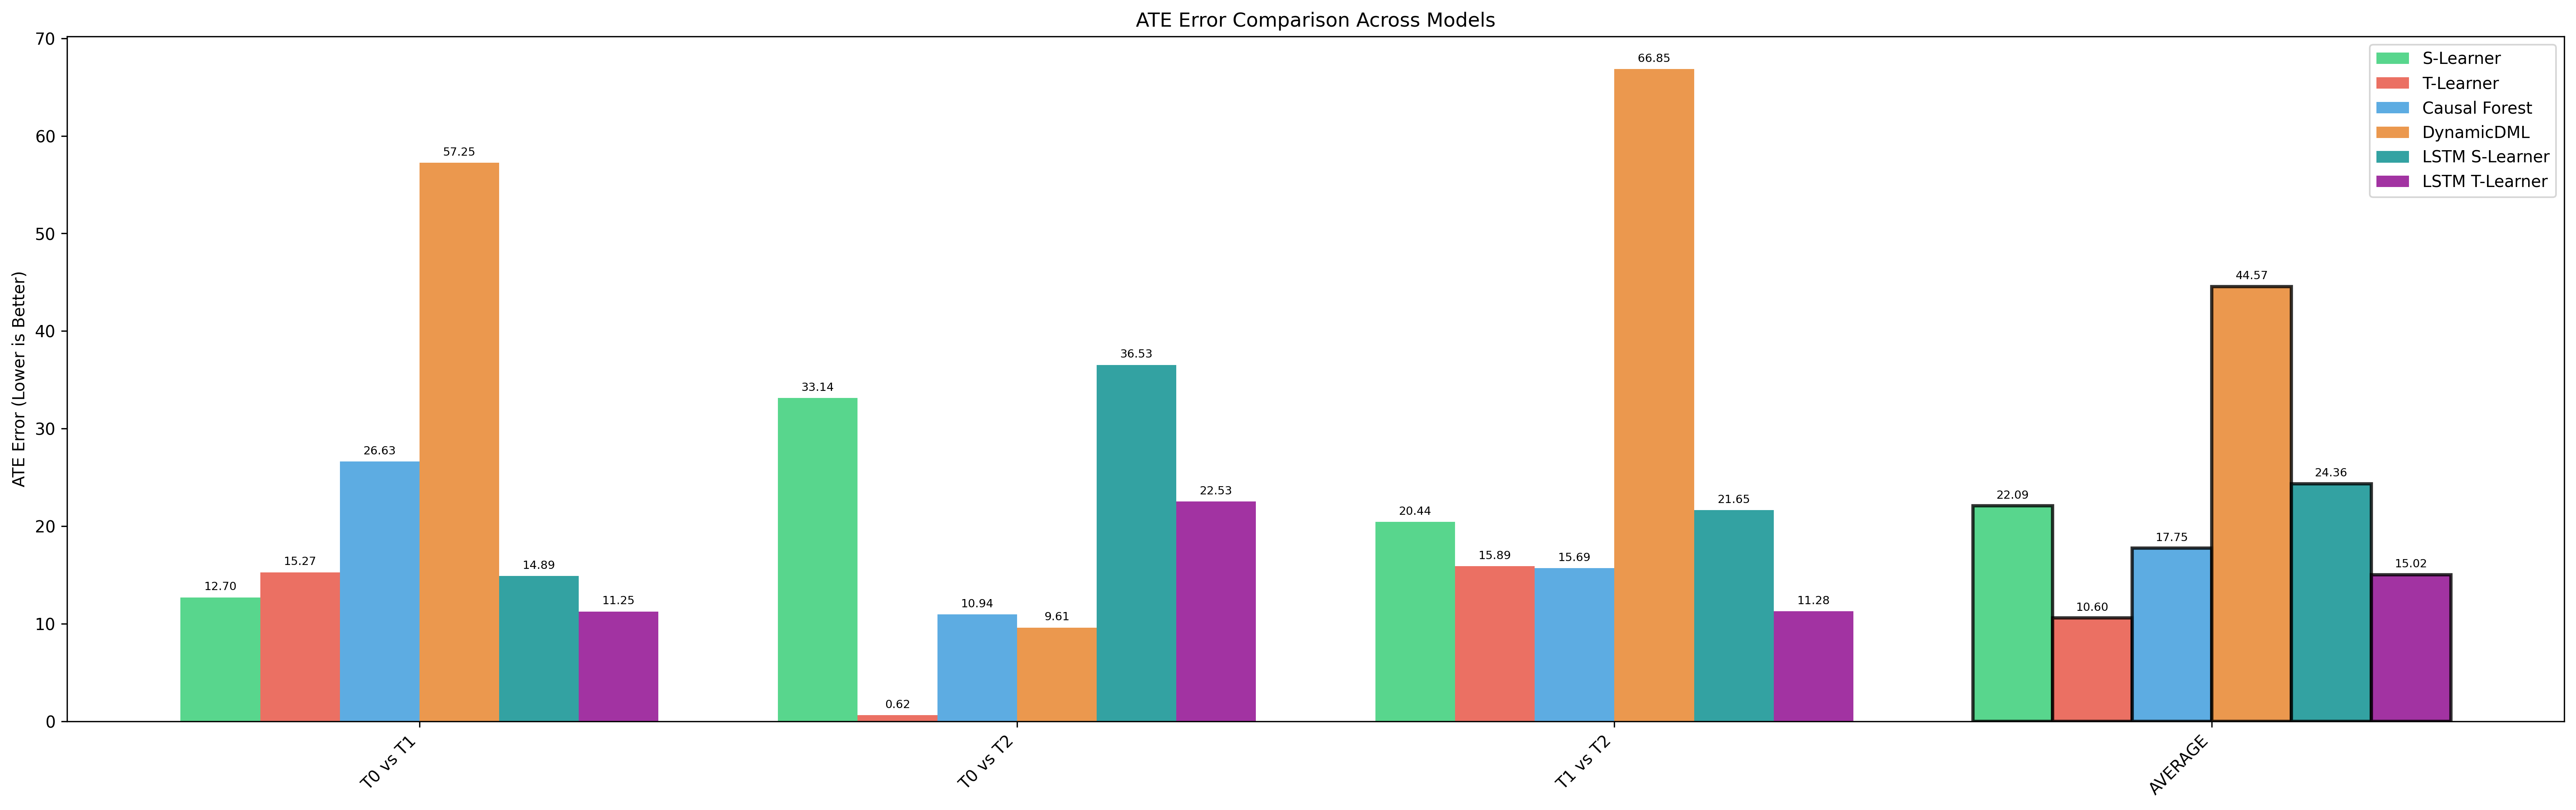
\includegraphics[width=\textwidth]{images/crn_pehe.png}
        \caption{PEHE by treatment pair (CRN labels)}
    \end{subfigure}
    \\
    \begin{subfigure}[b]{1\textwidth}
        \centering
        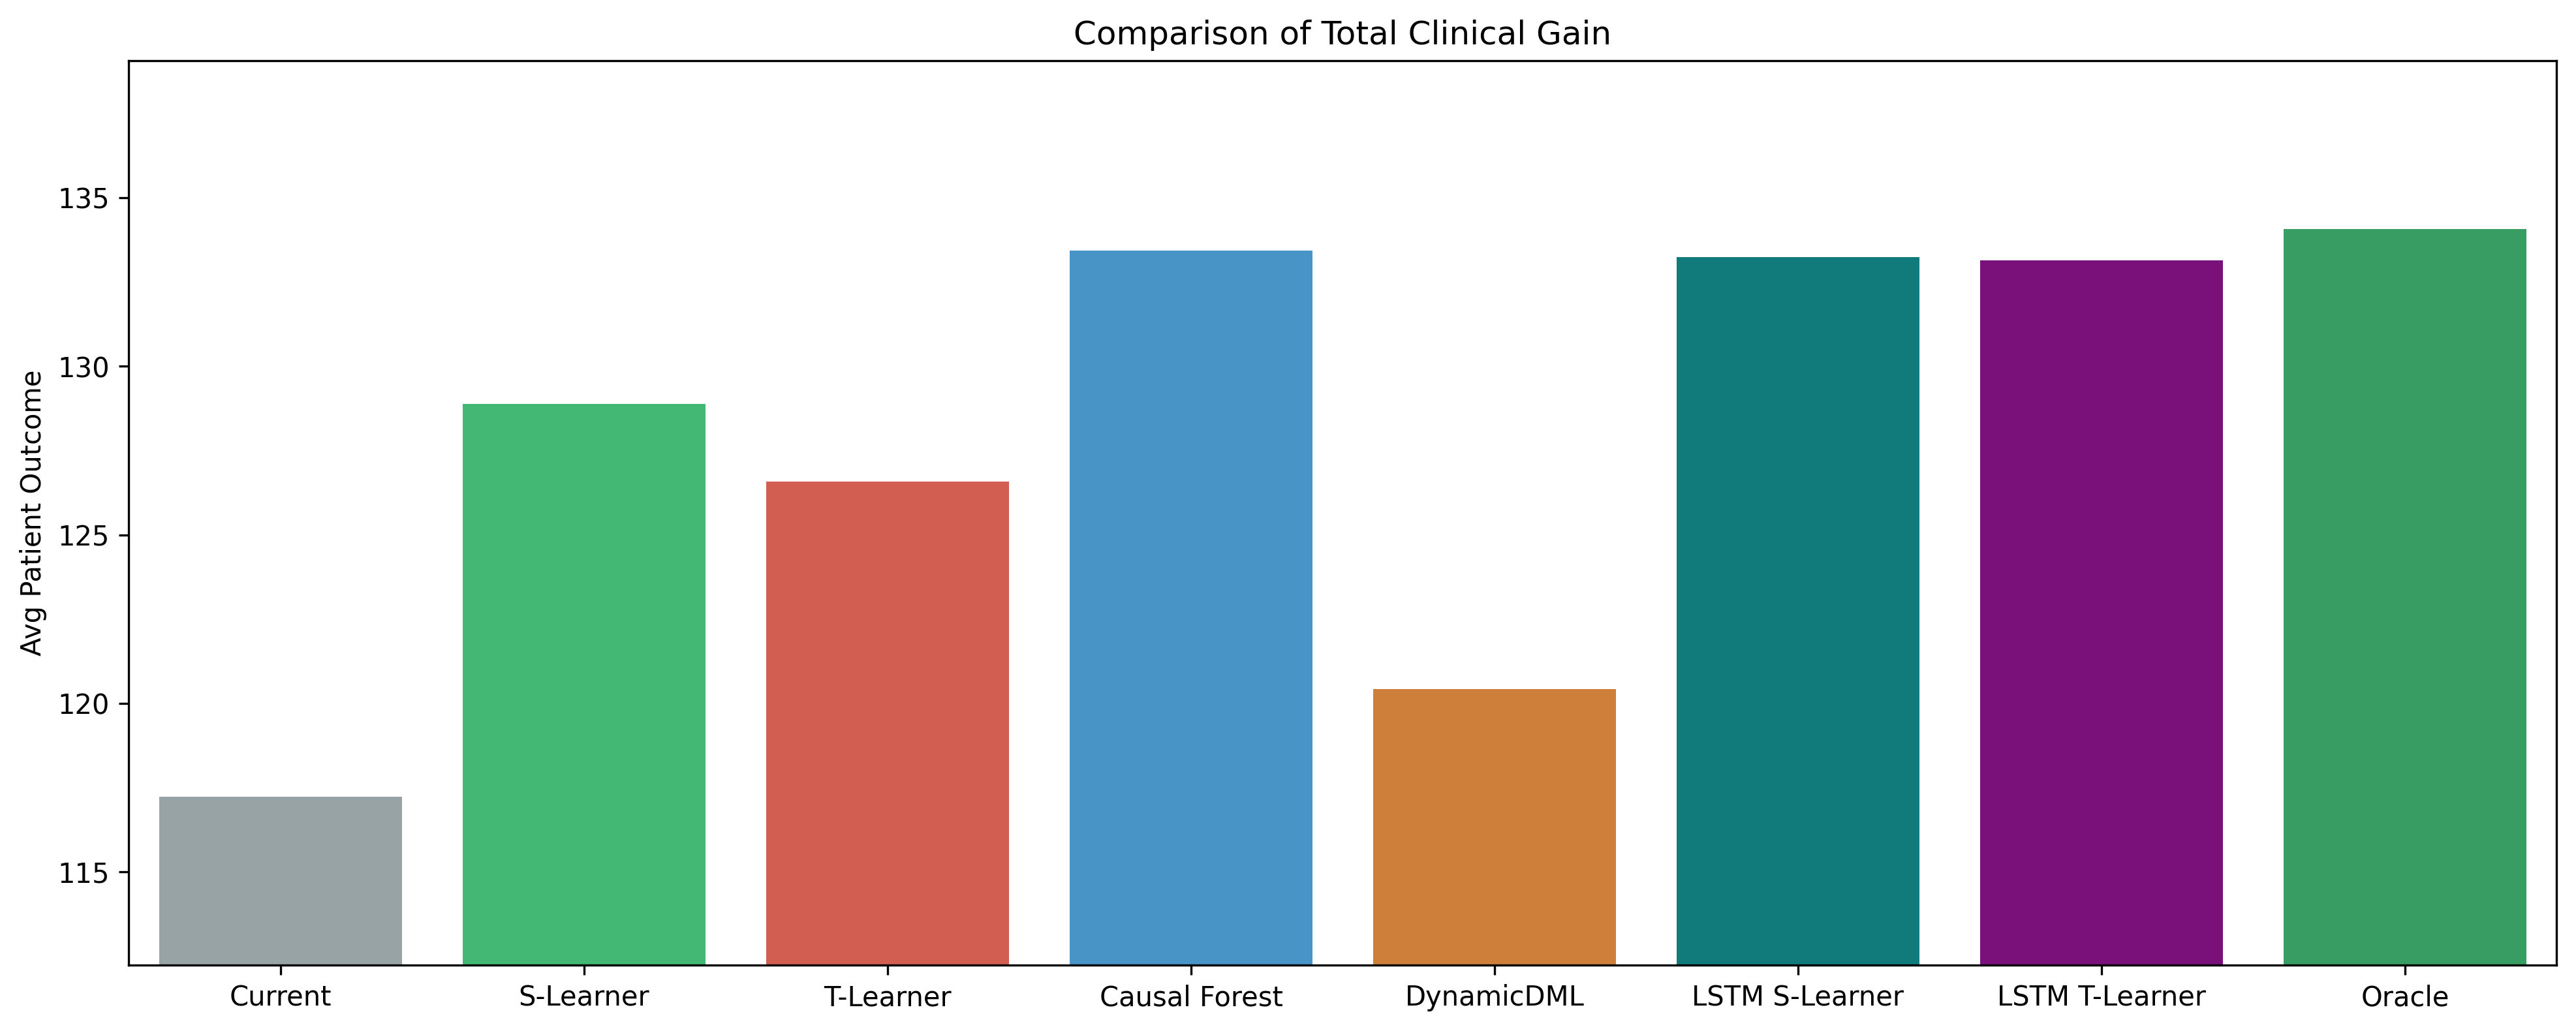
\includegraphics[width=\textwidth]{images/crn_policy.png}
        \caption{Policy value comparison (CRN labels)}
    \end{subfigure}
    \\
    \begin{subfigure}[b]{1\textwidth}
        \centering
        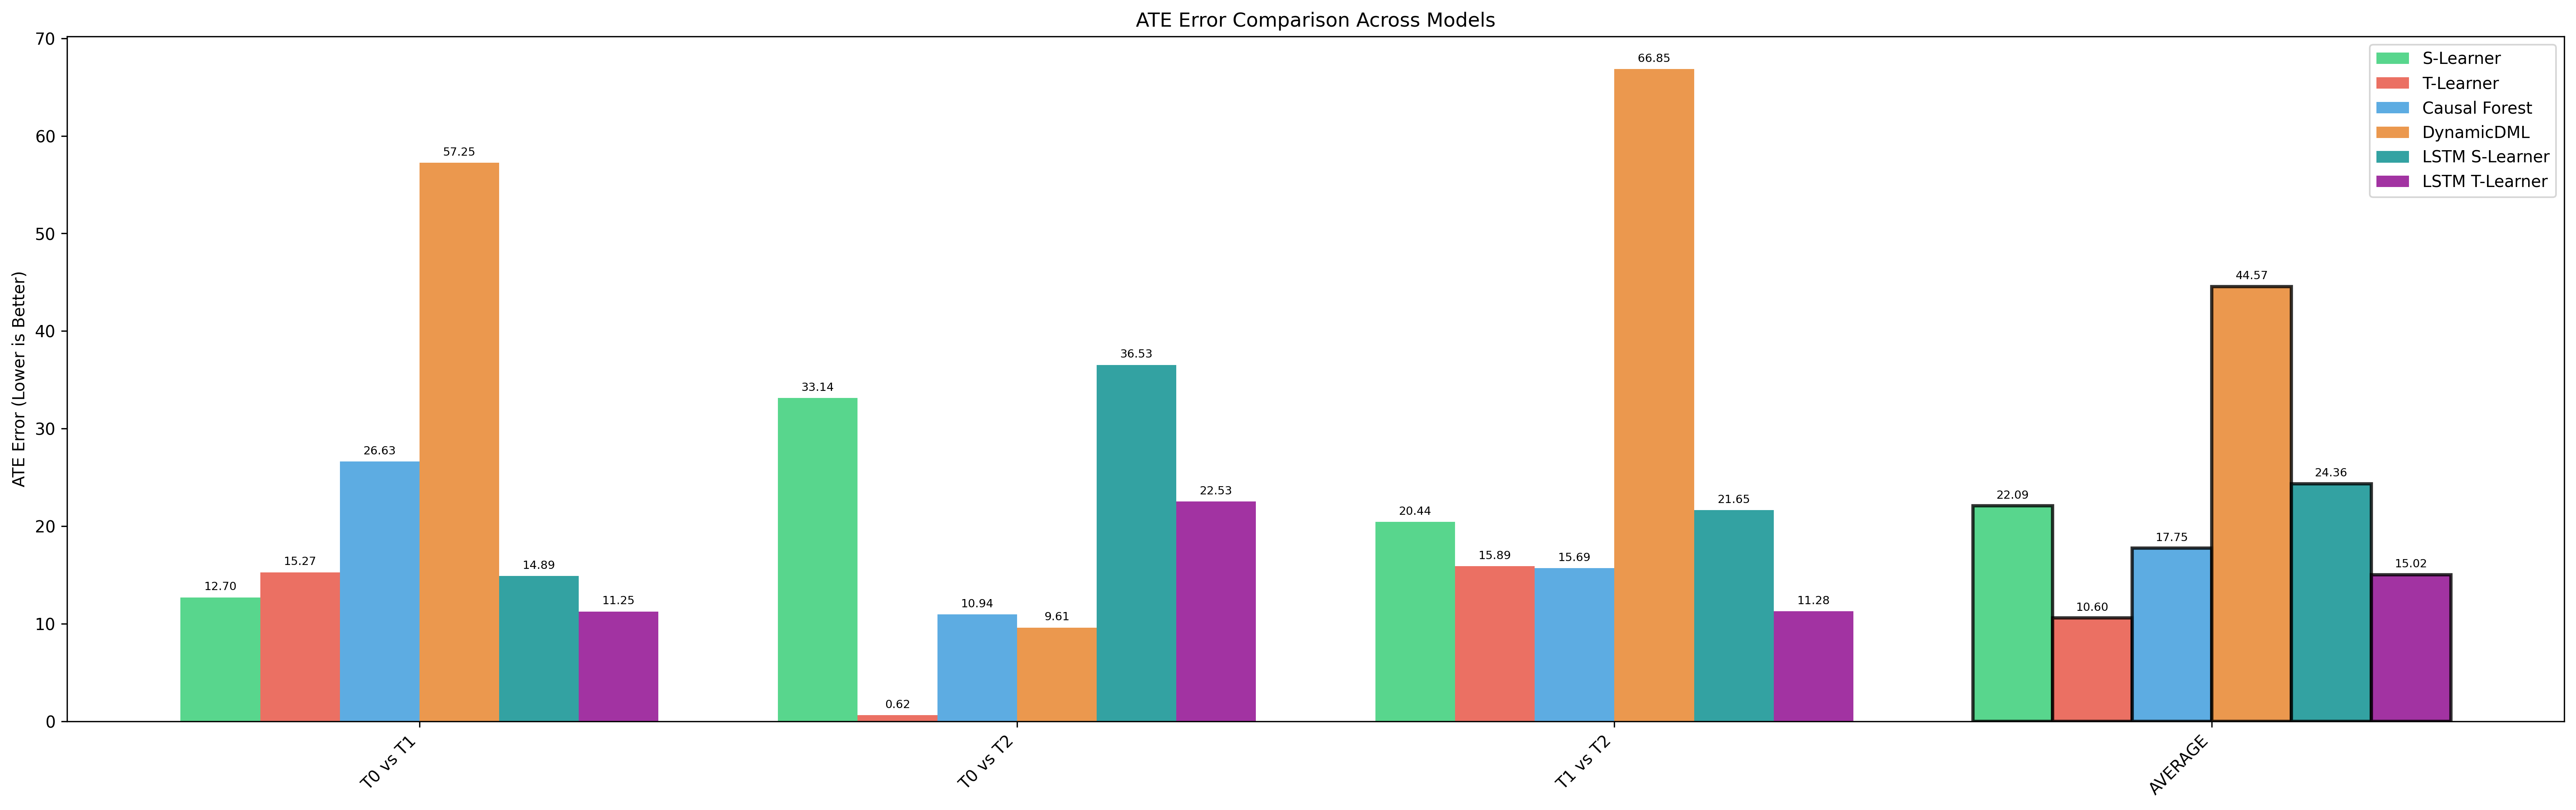
\includegraphics[width=\textwidth]{images/crn_ate.png}
        \caption{ATE error by treatment pair (CRN labels)}
    \end{subfigure}
    \caption{Model diagnostics on the CRN-based semi-synthetic evaluation set (18 test patients).}
    \label{fig:crn_model_plots}
\end{figure}

\newpage
\subsubsection{Fully synthetic generator results}

\label{sec:synth-results}
The fully synthetic evaluation uses 12\,000 training patients (77\,741 visit rows)
and 3\,000 test patients (19\,461 evaluation steps) generated by the synthetic
generator. All models are retrained from scratch on this split.

Recommendation accuracy and policy value are summarised in
Table~\ref{tab:synth_model_summary}. Dynamic DML achieves the highest recommendation
accuracy (70.4\%), followed by Causal Forest (61.7\%), BOWL (61.5\%), LSTM S-Learner
(60.7\%), LSTM T-Learner (59.4\%), T-Learner (58.3\%), and S-Learner (55.5\%). The
large sample setting directly benefits Dynamic DML: With approximately
38\,000 rows per cross validation fold the hunger for data is met, in contrast to the
small semi-synthetic training sets where Dynamic DML underperformed.
Policy values are tightly clustered between 244 and 248 days against an oracle of
251.04 and a random baseline of 238.20, with Dynamic DML achieving the highest
value (248.05).

For effect estimation, Dynamic DML also leads on PEHE ($T_0$ vs.\ $T_1$):
$\text{PEHE}_{01} = 15.41$, compared to Causal Forest (19.76), LSTM-T (19.22),
LSTM-S (20.05), T-Learner (23.09), and S-Learner (24.64).

Mean 95\% CI widths on the fully synthetic split are summarised in
Table~\ref{tab:synth_ci_width}. In this run, DynamicDML CI widths were contracted massively, while T-Learner remained the widest among the
available intervals and LSTM-T the tightest.

\begin{table}[H]
    \centering
    \begin{tabular}{lccc}
        \toprule
        \textbf{Model} & \textbf{CI width $T_0$\,v\,$T_1$} & \textbf{CI width $T_0$\,v\,$T_2$} & \textbf{CI width $T_1$\,v\,$T_2$} \\
        \midrule
        S-Learner     & 27.2856 & 42.1232 & 29.9185 \\
        T-Learner     & 234.4796 & 227.5683 & 224.3824 \\
        Causal Forest & 54.1061 & 49.1068 & 50.9114 \\
        Dynamic DML   & 31.1520 & 28.5244 & 29.2118 \\
        LSTM-S        & 28.1040 & 31.4609 & 27.6396 \\
        LSTM-T        & 11.6292 & 11.7814 & 10.4645 \\
        \bottomrule
    \end{tabular}
    \caption{Mean 95\% CI width on the fully synthetic evaluation set (19\,461 steps, 3\,000 patients).}
    \label{tab:synth_ci_width}
\end{table}

\begin{table}[H]
    \centering
    \begin{tabular}{lcccc}
        \toprule
        \textbf{Model} & \textbf{Accuracy} & \textbf{Policy Value} & \textbf{PEHE $T_0$\,v\,$T_1$} & \textbf{ATE err $T_0$\,v\,$T_1$} \\
        \midrule
        Dynamic DML   & 70.4\% & 248.05 & 15.41 & 0.32  \\
        Causal Forest & 61.7\% & 245.79 & 19.76 & 1.83  \\
        BOWL          & 61.5\% & 245.96 & --    & --    \\
        LSTM-S        & 60.7\% & 245.38 & 20.05 & 4.90  \\
        LSTM-T        & 59.4\% & 245.35 & 19.22 & 2.35  \\
        T-Learner     & 58.3\% & 244.97 & 23.09 & 0.21  \\
        S-Learner     & 55.5\% & 244.05 & 24.64 & 12.42 \\
        \midrule
        Oracle        & --      & 251.04 & --    & --    \\
        Random        & --      & 238.20 & --    & --    \\
        \bottomrule
    \end{tabular}
    \caption{Model summary on the fully synthetic evaluation set (19\,461 steps, 3\,000 patients). PEHE and ATE error are shown for the $T_0$ vs.\ $T_1$ treatment pair.}
    \label{tab:synth_model_summary}
\end{table}

Figure~\ref{fig:synth_model_plots} shows the PEHE comparison, policy value
diagnostics, and ATE error comparison. On this scale, Dynamic DML consistently
outperforms the other estimators: it achieves the lowest PEHE, the highest
policy value confirming that given sufficient data the panel DML estimator is well
suited to the treatment ranking task. The T-Learner achieves a low ATE error
(0.21 days) but ranks lower on policy value and PEHE.

\begin{figure}[H]
    \centering
    \begin{subfigure}[b]{1\textwidth}
        \centering
        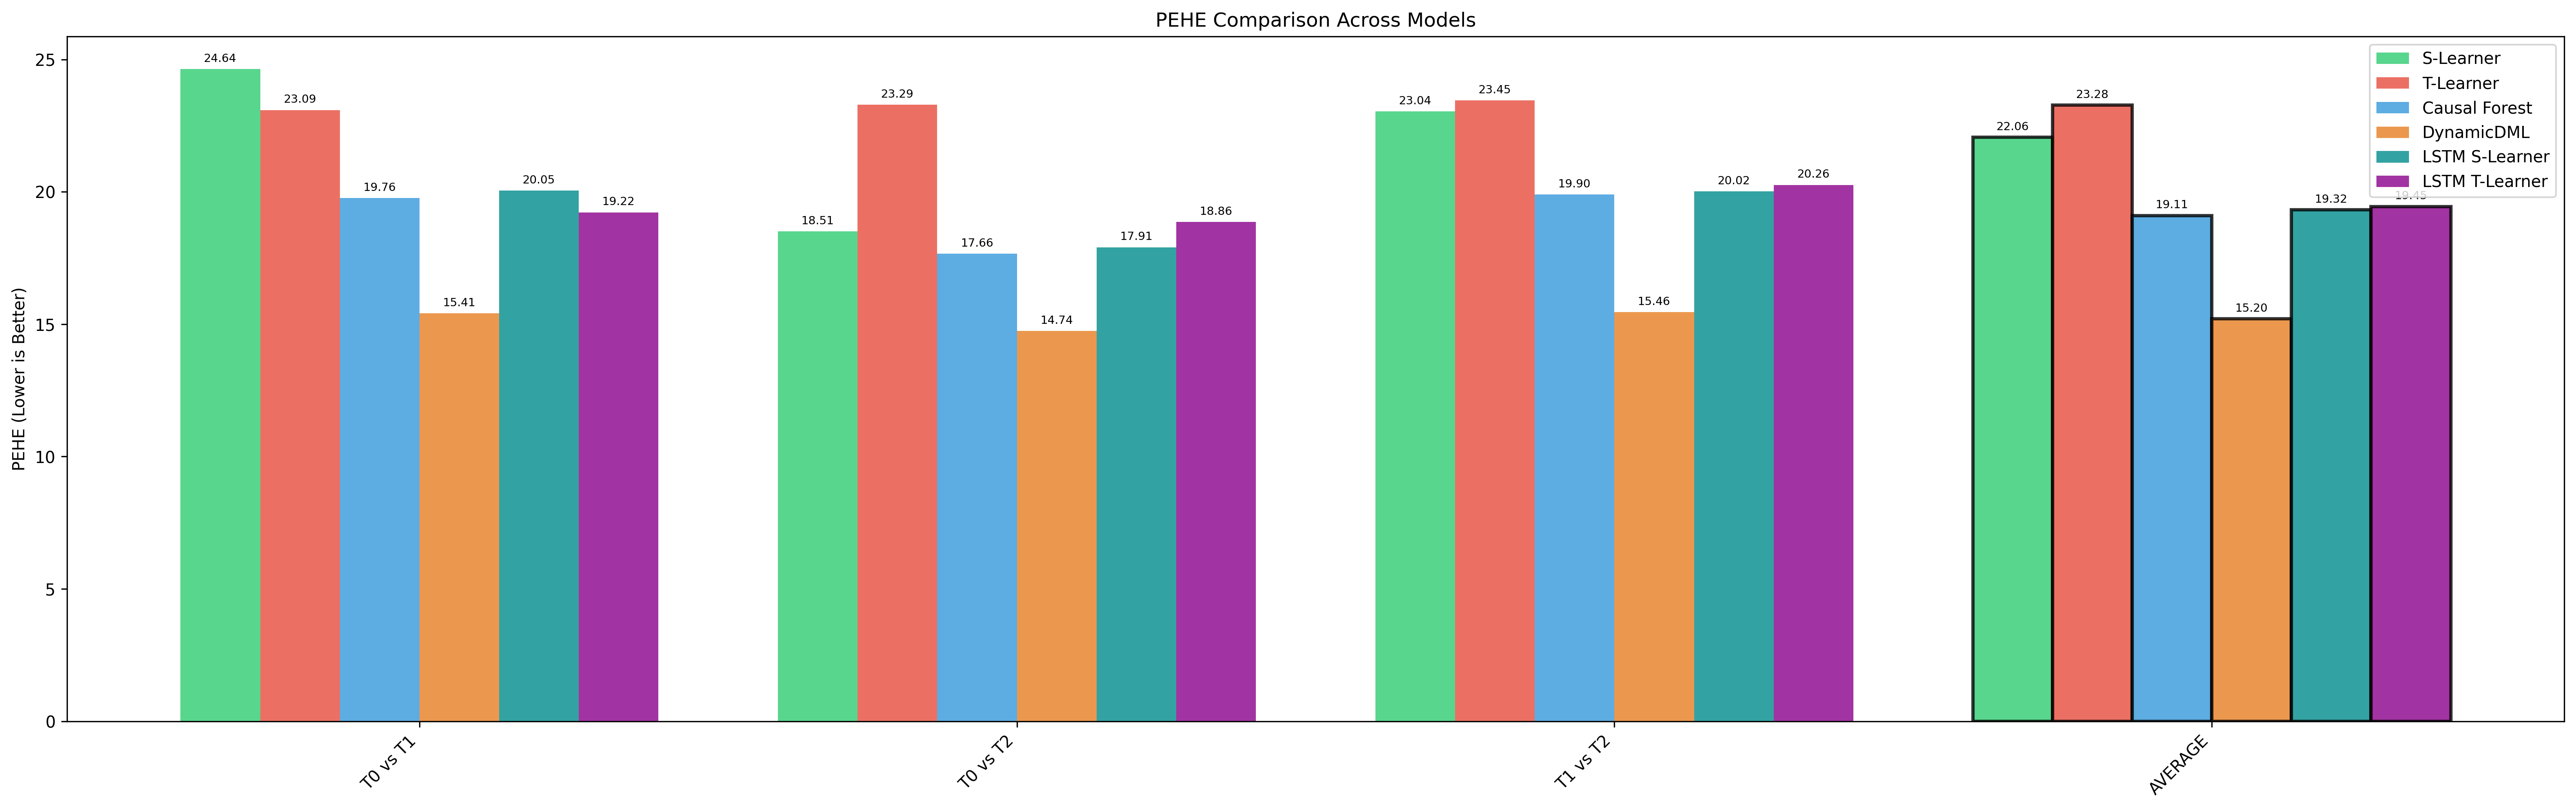
\includegraphics[width=\textwidth]{images/synth_pehe.png}
        \caption{PEHE by treatment pair}
    \end{subfigure}
    \\
    \begin{subfigure}[b]{1\textwidth}
        \centering
        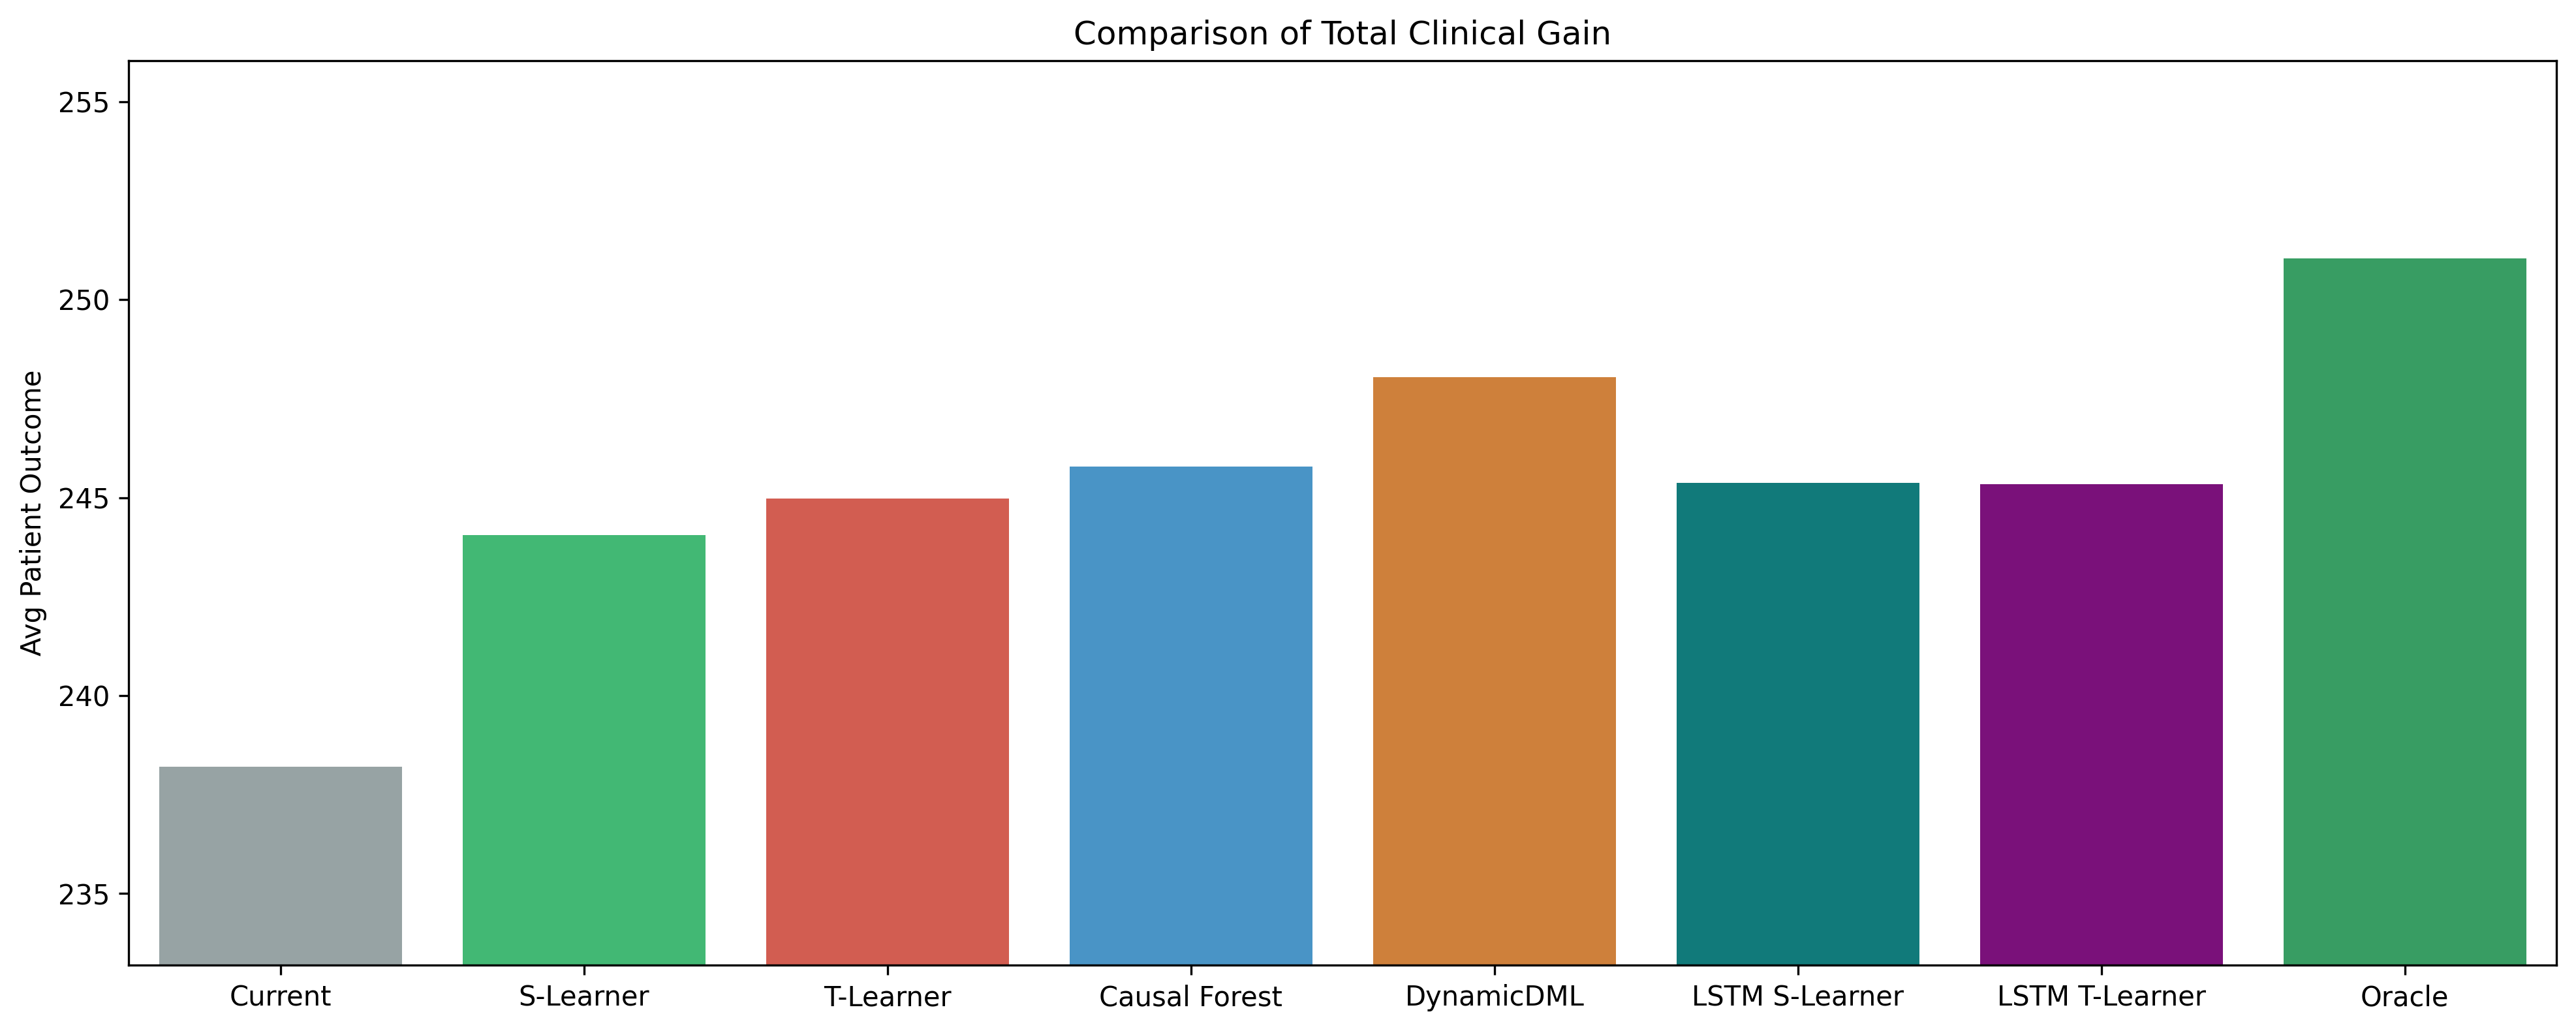
\includegraphics[width=\textwidth]{images/synth_policy.png}
        \caption{Policy value comparison}
    \end{subfigure}
    \\
    \begin{subfigure}[b]{1\textwidth}
        \centering
        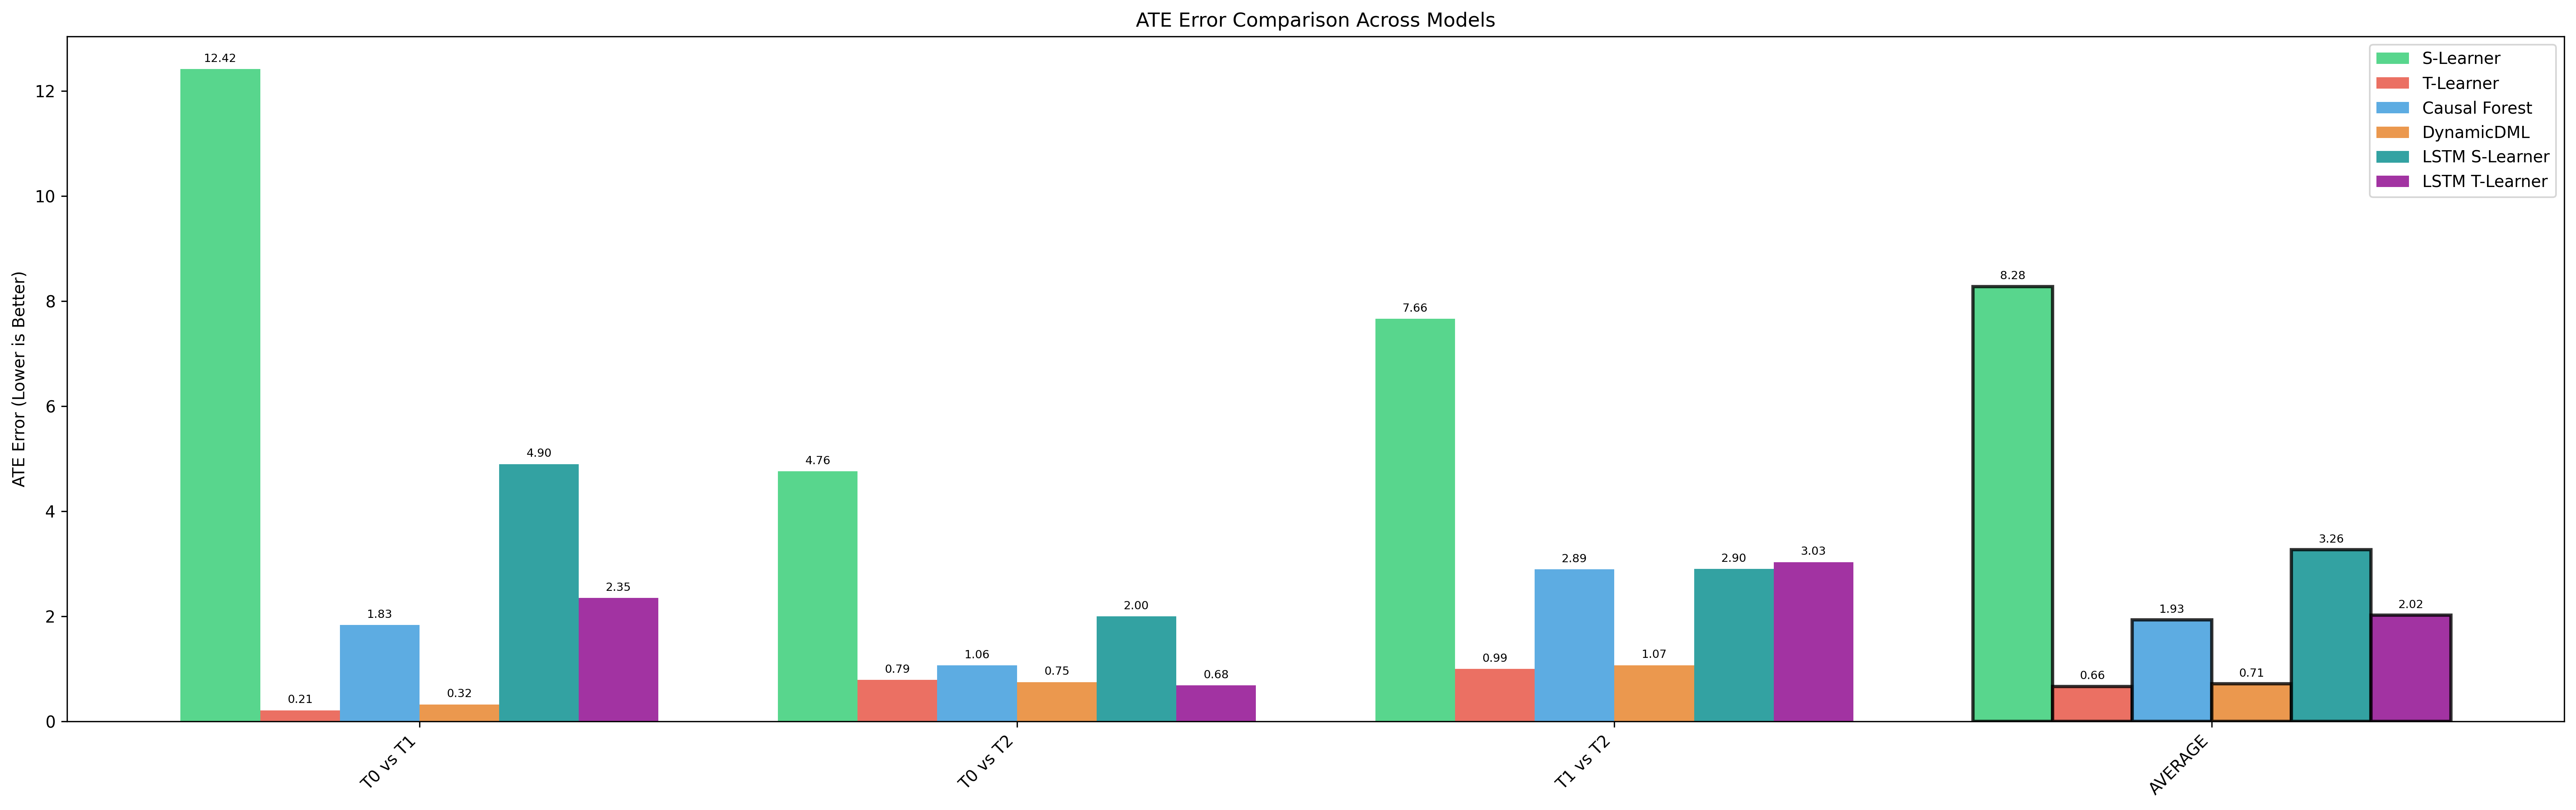
\includegraphics[width=\textwidth]{images/synth_ate.png}
        \caption{ATE error by treatment pair}
    \end{subfigure}
    \caption{Fully synthetic model diagnostics (3\,000 test patients).}
    \label{fig:synth_model_plots}
\end{figure}

\newpage
\section{Discussion}
\paragraph{Small sample size}
The 88-patient cohort is the single largest factor shaping the real-data results. With only 97 evaluation visits from 18 patients, a 10 percentage point difference in recommendation accuracy corresponds to roughly 10 visits being classified differently. The CRN-based and equation-based evaluations therefore carry substantial sampling variance, and apparent rankings between estimators should be read with that in mind. The fully synthetic regime removes this limitation and evaluates the estimators in a stable environment.

\paragraph{DynamicDML}
Dynamic DML is the most affected estimator by the small sample size. On
both real data regimes it has the lowest recommendation accuracy
(29.9\% on the equation-based generator, 51.5\% on the CRN-based one). On the fully
synthetic dataset however, the same estimator becomes the best
performer, reaching 70.4\% accuracy.
As discussed in
Section~\ref{sec:res-eu}, this difference is not a contradiction.
Dynamic DML requires its nuisance models to converge at a rate that the
70 patient training set cannot satisfy, but which is comfortably met
by the 12\,000-patient synthetic split. Dynamic DML is therefore best
characterised as an estimator that punishes data scarcity
heavily.

\paragraph{Uncertainty intervals}
The interval width results reinforce the scale effect and the estimator-specific
uncertainty behavior.
Across the equation-based semisynth split, DynamicDML and T-Learner
produce the widest intervals, Causal Forest is in the middle, and the LSTM
variants are the narrowest. On the fully synthetic run, interval widths
generally contract for the available models, but T-Learner remains broad.
Interval width should therefore be interpreted together with PEHE and ATE error,
not as a stand-alone ranking criterion.

\paragraph{LSTM vs.\ non-sequential variants}
On the CRN-based generator the LSTM-S Learner reaches 97.9\%
recommendation accuracy and the LSTM T-Learner 93.8\%, substantially
above the non-sequential S- and T-Learners at 68\% and 62\%. On the
equation-based regime this gap is much smaller, and on the fully
synthetic regime the LSTM variants and their non-sequential counterparts
are roughly tied. The CRN-based result therefore does not directly show that
sequential estimators outperform aggregated history estimators on
temporal data. The fully synthetic regime contains the same kind of
temporal structure, and the LSTM does not dominate there. A more
honest reading is that the CRN-based generator and the LSTM-based
estimators share an LSTM architecture, so the counterfactuals the CRN
produces are easier for the LSTM-based estimators to recover than for
the non-sequential baselines. The architectural similarity between
generator and estimator inflates the apparent LSTM advantage on the
CRN-based evaluation.

\paragraph{Semi-synthetic data}
The equation-based generator encodes handwritten parameters, so an
estimator's success on it primarily reflects how well it can recover
the structure built in by hand. The CRN learns its outcome dynamics
from the real factual outcomes and therefore carries more weight as
evidence about which estimators recover realistic counterfactual
structure. The LSTM-based metalearners strong performance under the
CRN evaluation is partly explained by their shared architecture,
as discussed above, but still indicates that sequence-aware estimators
can recover the counterfactual structure that a sequence-aware
generator extracts from real data.


\paragraph{BOWL}
BOWL performs consistently across the different evaluation regimes and
generally remains in the middle of the estimator rankings. Since BOWL
directly predicts a treatment policy rather than potential outcomes,
PEHE and ATE error are not defined for it. Its recommendation accuracy
however, varies less strongly between the CRN-based and fully synthetic
evaluations. This suggests that BOWL
is comparatively robust in low-data settings. At the same time, its performance
does not reach the highest accuracies.

\paragraph{Causal Forest}
The Causal Forest is the most consistent estimator across all evaluation
regimes and ranks among the top-performing models in every setting,
although it is never the single best performer. Unlike Dynamic DML, its
performance does not collapse under small sample sizes, and unlike the
LSTM-based estimators, it does not appear to benefit strongly from
architectural similarity to a specific generator. If a single estimator
had to be deployed without prior knowledge of the available data scale
or the underlying counterfactual structure, the Causal Forest would be
the most robust and defensible choice.

\paragraph{Assumptions}
The estimators rely on the identifying assumptions stated in
\Cref{sec:assumptions}, and the real-data results should be read in light of how
plausibly each holds here. Unconfoundedness is the most doubtful. It would require
that our feature set captures every factor that drives both the regimen choice and
the outcome, but the features are limited to ten EORTC QLQ-C30 subscales, gender,
diagnosis, and visit number. In practice, regimens are mainly chosen based on the
tumor stage, molecular markers, and the patient's general fitness. None of these are
in our feature set, so important hidden factors are missing and the estimated effects
are likely biased. Positivity is also shaky: with the arms split 46/18/36\% and only
438 training rows, some types of patient barely appear on certain arms, so the model
has little or no real example to compare against for those arms. Consistency is
weakened by the outcome itself, since \texttt{time\_to\_last\_days} mixes together
patients who finished treatment, died, or dropped out, so a longer value is not always
a better result.


\paragraph{Limitations}
The current implementation has multiple limitations that restrict the
generalisation of the results. The cohort is limited to lung cancer
patients receiving the three most frequent chemotherapy regimens, so
the findings may not transfer to other cancer types or less common
treatments. In addition, the regression target
\texttt{time\_to\_last\_days} acts only as a proxy for patient outcome
and is not a survival endpoint. The implementation
also considers only ten EORTC QLQ-C30 subscales, which limits the
amount of patient information available to the models.

\paragraph{Clinical implications}
The estimators implemented in this work can in principle support
personalised regimen ranking, but not at the cohort size analysed here.
The fully synthetic experiments show that panel-aware estimators are
capable of recovering heterogeneous treatment effects at sample sizes
of several thousand patients.

Future work could improve the quality of the estimated treatment
effects by using more clinically meaningful regression targets, such
as tumor size progression instead of \texttt{time\_to\_last\_days}. In addition,
including richer clinical features and longitudinal patient information
could allow the estimators to capture patient heterogeneity more
accurately and improve the realism of the generated counterfactual
outcomes.

\bibliographystyle{alpha}
\bibliography{sample}

\end{document}